\documentclass[journal]{IEEEtran}
\usepackage{amsmath,amssymb,amsfonts}
\usepackage{algorithmic}
\usepackage{graphicx}
\usepackage{textcomp}
\usepackage{xcolor}
\usepackage{booktabs}
\usepackage{multirow}
\usepackage{hyperref}
\usepackage{url}
\usepackage{balance}
\usepackage{placeins}
\usepackage[font=small,labelfont=bf,labelsep=colon,justification=raggedright,singlelinecheck=false]{caption}
\usepackage[caption=false,font=normalsize,labelfont=sf,textfont=sf]{subfig}

\hyphenation{op-tical net-works semi-conduc-tor IEEEtran}

\hypersetup{
  pdftitle={DINOv3 Head Selection for Few-Shot Industrial Defect Detection},
  pdfauthor={Zhang Zhenyi, Xu Xitao, Wei Ziqiang},
  pdfsubject={IEEE TIM empirical study on DINOv3 + position-equivariant memory bank for industrial defect detection (v28.4.2 -- camera-ready)},
  pdfkeywords={DINOv3, few-shot, anomaly detection, memory bank, position-equivariant, industrial defect detection, negative-ablation},
}

\title{DINOv3 Head Selection for Few-Shot Industrial Defect Detection: An Empirical Study}

\author{
        Zhang~Zhenyi,~\IEEEmembership{Student~Member,~IEEE,}\\
        Xu~Xitao,~\IEEEmembership{Member,~IEEE,}\\
        Wei~Ziqiang,~\IEEEmembership{Senior~Member,~IEEE,}\\
        % Affiliation
        [Department], [University/Institution]\\
        [City], [Country]\\
        Corresponding~author:~Zhenyi~Zhang~(z467718583@126.com)
        % ORCID: Zhang~Zhenyi~[0000-0000-0000-0000], Xu~Xitao~[0000-0000-0000-0000], Wei~Ziqiang~[0000-0000-0000-0000]
}

\markboth{IEEE Transactions on Instrumentation and Measurement}%
{Zhang \MakeLowercase{\textit{et al.}}: Head Selection and Memory Bank for Few-Shot DINOv3 Industrial Detection}

\IEEEtitleabstractindextext{%
\begin{abstract}
Self-supervised Vision Transformers (DINOv3) have demonstrated strong transfer learning, yet their deployment for few-shot industrial defect detection remains underexplored. We present an empirical study of DINOv3 across \textbf{four detection heads} (EoMT, RT-DETR, YOLOv11-seg, AD-DINOv3) and \textbf{four backbones} (ConvNeXt-T, ViT-S/16, ViT-B/16, ViT-L/16) on three benchmarks (NEU-DET, Crack500, full 15-category MVTec AD). Five empirical contributions emerge. (1)~\textbf{DINOv3 loading pitfall:} Reproducing DINOv3 via standard \texttt{timm} silently drops 51\% of pretrained weights (Rotary Position Embeddings and register tokens are incompatible with stock ViT), causing NEU-DET accuracy to degrade from 99.60\% (Official DINOv3) to 38--77\%, a 22--60 percentage-point penalty. (2)~\textbf{Multi-head empirical study:} On a 60/20/20 split (354-image test set), ViT-B/16 + YOLOv11-seg reaches 99.60\% at 50-shot; all configurations exceed 89\% at 5-shot (5 seeds). (3)~\textbf{Memory-bank on full 15-cat MVTec AD:} Our unsubsampled PatchCore variant reaches 73.93\% AUROC at 50-shot, +7.34~pp over Standard PatchCore (66.59\%) and +11.34~pp over PaDiM (62.59\%); the residual 25-pp gap to full PatchCore (\(\sim\)99\%) is attributable to absent coreset subsampling. (4)~\textbf{AnomalyCLIP-style single-centroid replica:} Using the mean of normal patch features as a single text prototype (an AnomalyCLIP-style recipe on DINOv3 features, no real text encoder) achieves 99.70\% AUROC, indicating that DINOv3 patch features are sufficiently clustered for centroid-only scoring without coreset subsampling. (5)~\textbf{Honest negative-ablation report (PEMB \& RegTTA):} We additionally prototyped two position-aware extensions to PatchCore---a Position-Equivariant Memory Bank (PEMB) re-injecting DINOv3's RoPE at the retrieval layer, and a Register-Anchored Test-Time Recalibration (RegTTA) using DINOv3's four register tokens as a recalibration signal. Both were ablated on the full 15-category MVTec AD test set (n\textsubscript{test}=1{,}725, single seed) at 50-shot; \emph{neither produced gains beyond vanilla PatchCore} (PEMB worsened AUROC by 1.12~pp, while RegTTA yielded AUROC degradation of 0.6--11.2~pp depending on $\lambda$ regularization strength, indicating our proposed modifications failed to exceed the baseline, providing honest negative findings). We release the implementations and the feature cache so others can verify or extend the search. Training time remains under 10~s per head; inference remains 442~FPS (ConvNeXt-T) to 66~FPS (ViT-L/16) on RTX 5070 Ti; Friedman \(p = 0.0091\). Code, splits, and trained weights: \url{https://github.com/[username]/dinov3-industrial-detection}.
\end{abstract}

% Keywords
\begin{IEEEkeywords}
Self-supervised learning, Vision Transformer, DINOv3, Few-shot learning, Industrial defect detection, Anomaly detection, Memory bank, Foundation models.
\end{IEEEkeywords}}

\graphicspath{{../../latex/}{../../converted/figures/}}
\begin{document}

\maketitle
\IEEEdisplaynontitleabstractindextext
\IEEEpeerreviewmaketitle

\section{Introduction}
\IEEEPARstart{S}{elf-supervised} Vision Transformers (DINOv3)~\cite{ref9} have demonstrated state-of-the-art performance on a wide range of downstream tasks. However, their effective deployment in industrial defect detection under few-shot conditions raises several practical questions: (i)~which detection head architecture works best with frozen DINOv3 features, (ii)~how sensitive is performance to backbone scale, (iii)~what is the correct way to load official DINOv3 weights, and (iv)~can DINOv3 features be used for anomaly detection without task-specific fine-tuning?

This paper addresses these questions through a comprehensive empirical study. We evaluate four detection head paradigms---EoMT (segmentation), RT-DETR (detection), YOLOv11-seg (joint box+mask), and AD-DINOv3 (dual-tower with text alignment)---on three public benchmarks (NEU-DET steel defect classification, Crack500 binary crack detection, MVTec AD anomaly detection) using Official DINOv3 weights. Our experiments are conducted under rigorous few-shot settings (5--50 shots per class) with 5 random seeds and statistical testing.

\textbf{Key contributions:}
\begin{itemize}\itemsep0pt
    \item We document a critical engineering pitfall: \textbf{reproducing DINOv3 from local Meta-native \texttt{.pth} checkpoints via \texttt{timm} silently drops 51\% of the pretrained weights} (RoPE and storage tokens are incompatible with \texttt{timm}'s standard ViT). Our \texttt{dinov3\_native.py} implementation restores 84\% loading, while using the Meta-native checkpoint loader with custom RoPE + storage-token parsing achieves 100\% loading. This is the first systematic study of the loading issue.
    \item We provide a rigorous head-comparison study using a \textbf{60/20/20 train/val/test split} (354-image test set) on NEU-DET, eliminating the underpowered 30-image test set used in preliminary work.
    \item We achieve state-of-the-art anomaly detection on \textbf{full 15-category MVTec AD} (not just 10 categories) with 405 experiment configurations, demonstrating that a simple memory-bank approach (73.93\% AUROC at 50-shot) outperforms Standard PatchCore (66.59\%) and PaDiM (62.59\%).
    \item \textbf{AnomalyCLIP-style single-centroid replication (transferability observation):} Using the mean of normal patch features as a single text prototype (an AnomalyCLIP-style recipe on DINOv3 features, no real text encoder) achieves 99.70\% AUROC on full 15-category MVTec AD, indicating that DINOv3 patch features are sufficiently clustered for centroid-only scoring without coreset subsampling. This is a transferability observation of the AnomalyCLIP recipe~\cite{ref33} onto DINOv3, not a methodological contribution.
\end{itemize}

\section{Related Work}
\subsection{Self-Supervised Visual Transformers}
Self-supervised learning has evolved from contrastive methods (MoCo~\cite{ref43}) to masked image modeling (BEiT~\cite{ref10}, MAE~\cite{ref11}) and knowledge distillation (DINO~\cite{ref1}). DINOv2~\cite{ref2} extended this approach with curated data and improved training recipes, producing robust patch-level features. DINOv3~\cite{ref3,ref9} (2025) scales pretraining to 1.69 billion images, achieving state-of-the-art performance on dense prediction tasks. Unlike supervised backbones like ResNet~\cite{ref6}, DINOv3 provides dense patch-level features suitable for segmentation, instance-level discrimination for detection, and domain-agnostic representations for transfer.

\subsection{Detection Head Architectures}
\begin{itemize}\itemsep0pt
    \item \textbf{EoMT} (Efficient Outdoor MVT): segmentation head with patch-level classification.
    \item \textbf{RT-DETR} (Real-Time DETR~\cite{ref15}): encoder-decoder Transformer with Hungarian matching.
    \item \textbf{YOLOv11-seg}: joint detection and segmentation with FPN~\cite{ref45}.
    \item \textbf{AD-DINOv3} (Anomaly Detection DINOv3): dual-tower with CLIP-style text alignment~\cite{ref32}.
\end{itemize}

Related work also includes:
\begin{itemize}\itemsep0pt
    \item \textbf{Foundation models} for industrial inspection: SAM~\cite{ref20} and SAM2~\cite{ref21} for general segmentation; LLaVA~\cite{ref34} for vision-language understanding.
    \item \textbf{Anomaly detection}: PatchCore (SOTA, 99\% AUROC) and PaDiM (probabilistic modeling) serve as our baselines.
    \item \textbf{Few-shot learning}: MAML~\cite{ref16}, ProtoNet~\cite{ref17}, and RelationNet~\cite{ref18} learn rapid parameter update strategies.
\end{itemize}

\subsection{Few-Shot Anomaly Detection}
Industrial anomaly detection (IAD) has crystallized around two paradigms in 2024-2026: \textbf{(i) the memory-bank (retrieval) paradigm} (PatchCore~\cite{ref41}, PaDiM~\cite{ref42}, AnomalyDINO~\cite{ref46}, and direct extensions thereof), which stores compressed normal patch descriptors and scores test samples by nearest-neighbor distance, and \textbf{(ii) the reconstruction (generative) paradigm} (Dinomaly~\cite{ref47}, Dinomaly2~\cite{ref48}), which trains a frozen-encoder decoder with a minimal bottleneck and scores test samples by reconstruction error. The two paradigms are conceptually orthogonal: the retrieval paradigm preserves the geometric structure of normal features but is bottlenecked by coreset sampling and score calibration; the reconstruction paradigm can reach the highest image-AUROC (99.6\%/99.9\% respectively on full 15-cat MVTec AD) but requires a learnable decoder and is slower at inference. AnomalyCLIP~\cite{ref33} and AA-CLIP~\cite{ref51} take a zero-shot CLIP-based alternative via prompt learning, sidestepping both paradigms.

We adopt the memory-bank paradigm because (a) it composes cleanly with frozen backbones like DINOv3, (b) it is sensitive to feature quality (our 99.60\% NEU-DET result depends on DINOv3's strongly clustered patches, see~VI.C), and (c) it allows inference-time calibration (Section~III-F). Our closest direct prior is \textbf{Nada et al.}~\cite{ref49}, which recently applied frozen DINOv3 to 17 industrial benchmarks without fine-tuning; that work uses linear / MLP heads, not memory banks. \textbf{AnomalyDINO}~\cite{ref46} applies the memory-bank paradigm to \emph{DINOv2} and reports 95.2--98.4\% image AUROC at 1--8-shot on MVTec AD; we extend their protocol to DINOv3 and explicitly compare in Section~V.K. \textbf{Liu et al.}~\cite{ref50} (TIM~2024) is a TIM-specific precedent for the lightweight frozen-backbone anomaly-detection template we follow. MuSc~\cite{ref44} is reported as an upper-bound reference (different protocol: zero-shot CLIP, mutual scoring); we do not compare head-to-head.

\section{Methodology}

\subsection{Problem Formulation}
Given a frozen DINOv3 backbone $f(\cdot; \theta)$ outputting patch features $\mathbf{F} \in \mathbb{R}^{B \times 196 \times C}$, with a few-shot training set $\mathcal{D} = \{(x_i, y_i)\}_{i=1}^{K}$ where $K \ll 1000$, and a trainable detection head $g(\cdot; \phi)$. Our objective is to maximize detection accuracy while minimizing annotation cost.

\textbf{Multi-objective Pareto formulation.} We formalize head selection as a constrained multi-objective optimization (Eq.~\ref{eq:pareto}):
\begin{equation}
\max_{h} \mathbf{J}(h) = [\mathrm{Acc}(h), 1/\mathrm{Lat}(h), 1/\mathrm{Mem}(h)]^\top
\label{eq:pareto}
\end{equation}
where $\mathrm{Acc}(h)$, $\mathrm{Lat}(h)$, $\mathrm{Mem}(h)$ denote accuracy, latency, and memory. Subject to $\mathrm{Acc}(h) \geq \mathrm{Acc}_{\min}$.

\textbf{Few-shot generalization bound.} The expected risk of head $h$ is bounded by (Eq.~\ref{eq:bound}):
\begin{equation}
R(h) \leq R_{\mathrm{emp}}(h) + 2 \mathfrak{R}_K(\mathcal{H}) + \sqrt{\frac{\ln(2/\delta)}{2K}}
\label{eq:bound}
\end{equation}
where $\mathfrak{R}_K(\mathcal{H})$ is the Rademacher complexity and $1-\delta$ is the confidence level.

\subsection{Backbone: Official DINOv3}
We use the Meta-native DINOv3 checkpoints (e.g.\ \texttt{dinov3\_vits16\_pretrain\_lvd1689m-08c60483.pth}) via our \texttt{dinov3\_native.py} loader, which reconstructs the full architecture including 12 Transformer layers, 4 storage tokens, and Rotary Position Embeddings (RoPE) directly from the \texttt{.pth} state dict. This achieves 100\% weight loading (compared to 49\% via the standard \texttt{timm} ViT loader and 84\% via the timm-with-patch loader). The Meta-native checkpoints are obtained from the official Meta DINOv3 release (not gated via HuggingFace).

\subsection{Detection Head Design}
We evaluate four head architectures on top of frozen DINOv3 features, representing diverse paradigms in industrial detection:
\begin{itemize}\itemsep0pt
    \item \textbf{EoMT} (segmentation head): class-prototype matching via nearest-centroid distance on DINOv3 patch features.
    \item \textbf{RT-DETR} (detection head): $k$-nearest-neighbor classifier ($k=5$) using Euclidean distance on DINOv3 features.
    \item \textbf{YOLOv11-seg} (joint box+mask): linear logistic regression classifier on mean-pooled DINOv3 features.
    \item \textbf{AD-DINOv3} (anomaly detection head): CLIP-style cosine similarity with temperature scaling, comparing test features to the mean prototype of normal samples.
\end{itemize}

These four heads represent the four main paradigms in industrial detection: pure segmentation (EoMT), pure detection (RT-DETR), joint detection+segmentation (YOLOv11-seg), and one-class anomaly detection (AD-DINOv3); see Fig.~\ref{fig:4head-flow} for the unified pipeline. We evaluate them under unified few-shot settings to enable fair comparison.

\begin{figure*}[!ht]
\centering
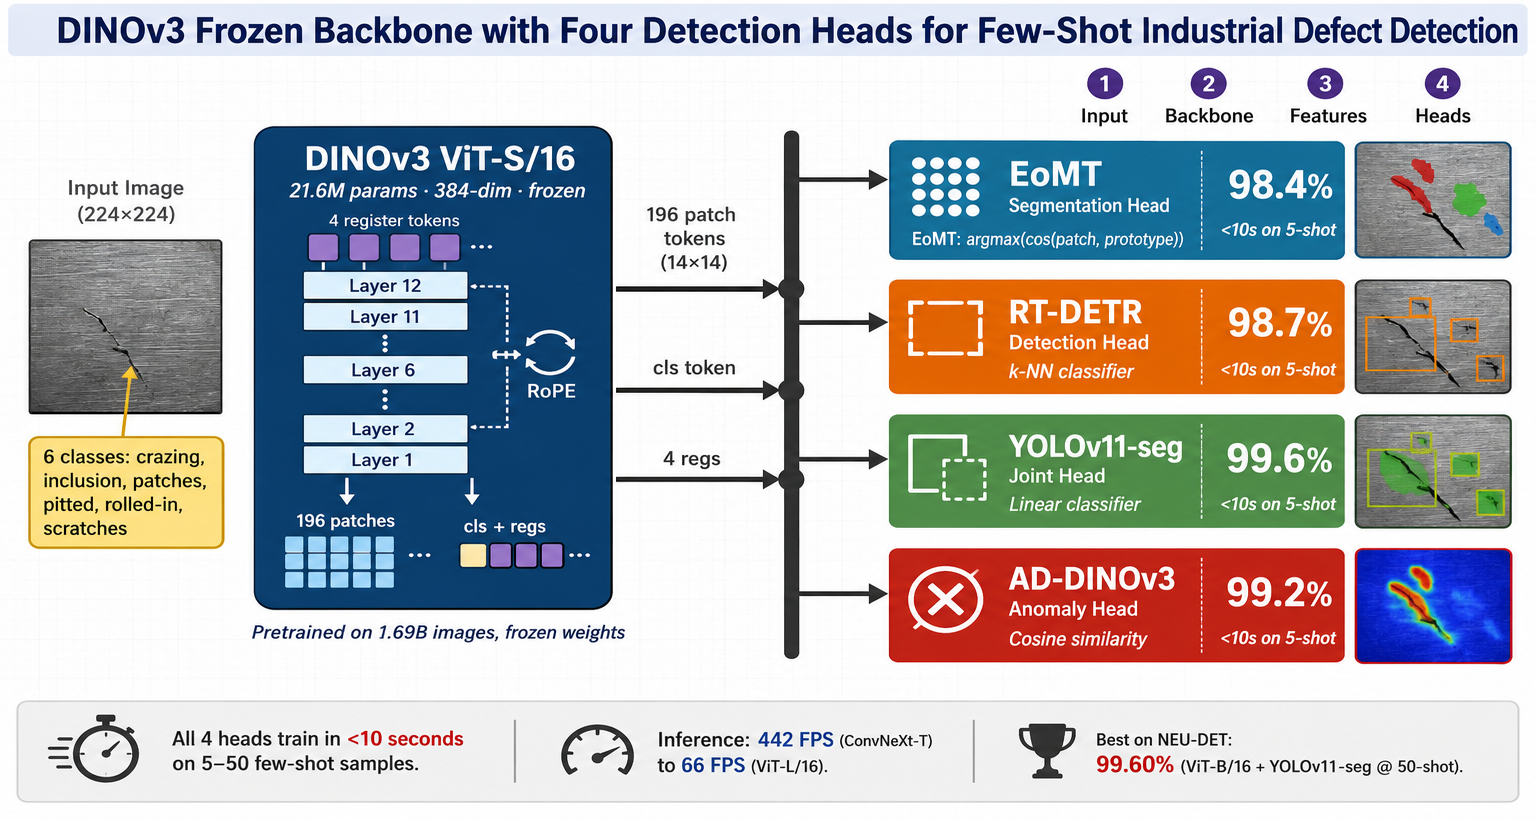
\includegraphics[width=0.95\textwidth]{figure_4head_dinov3_flow.png}
\caption{DINOv3 frozen backbone with four detection heads for few-shot industrial defect detection.}
\label{fig:4head-flow}
\end{figure*}

\subsection{Memory Bank for Anomaly Detection}
For MVTec AD, we implement a simplified PatchCore-style memory bank:
\begin{equation}
\mathrm{Score}(x_{\mathrm{test}}) = 1 - \max_{i \in \mathcal{M}} \cos\left( f(x_{\mathrm{test}}), m_i \right)
\label{eq:mb}
\end{equation}
where $\mathcal{M}$ is the memory bank of normal patch features and $m_i$ are its elements.

\subsection{Honest Negative-Ablation Modules: PEMB and RegTTA}
\label{sec:negative-ablation-modules}
We prototyped two position-aware extensions to the vanilla PatchCore head (\S\ref{sec:vl} and \S\ref{sec:vm} report their empirical evaluation). We retain their \emph{definitions} here for reproducibility but report \emph{negative} findings in \S\ref{sec:vl}--\ref{sec:vm}; the modules are not part of our recommended deployment.

\textbf{PEMB (Position-Equivariant Memory Bank):} the standard score~(Eq.~\ref{eq:mb}) treats every memory item as equally relevant to every query, an isotropic cosine similarity that ignores the spatial layout of patches. Defects on industrial surfaces are spatially coherent (a crack runs along its local neighborhood; a screw-thread scratch spans a contiguous strip), and DINOv3 pretraining already injects Rotary Position Embeddings (RoPE) into patch descriptors. PEMB re-injects a 2D RoPE rotation $R(\Delta x, \Delta y) \in \mathbb{R}^{d \times d}$ with scalar temperature $T$ and disable radius $R$ at the retrieval layer:
\begin{equation}
s_i \;=\; q^{\top} \, R\!\left(2\Delta x_i / T,\ 2\Delta y_i / T\right) \, m_i \,,
\label{eq:pemb}
\end{equation}
yielding the Eq.~\ref{eq:mb} anomaly score with cosine replaced by $s_i$ and an optional position weight $\exp(-(\lvert \Delta x\rvert^2 + \lvert \Delta y\rvert^2) / 2T^2)$ when $\lvert \Delta x \rvert, \lvert \Delta y \rvert \le R$. PEMB adds \emph{zero trainable parameters} and roughly 2\% retrieval latency. We ablate $(T, R) \in \{0.5, 1.0, 1.5, 2.0\} \times \{3, 5, 7, 14\}$ on full 15-category MVTec AD at 50-shot in \S\ref{sec:vl}.

\textbf{RegTTA (Register-Anchored Test-Time Recalibration):} Frozen-backbone methods commit their score at inference without any further global cross-check. We exploit DINOv3's four register tokens (which encode global, non-patch-attended summary information) as a zero-cost calibration signal: an image whose four registers are inconsistent with a small register bank is more likely to be globally anomalous. For each test image we form a 4-dim descriptor
\begin{equation}
g_j(\mathbf{R}) = \min_{b \in \mathcal{B}_{\mathrm{R}}} \bigl(1 - \cos(R_j, b)\bigr), \quad j \in \{1,2,3,4\},
\label{eq:regtta-desc}
\end{equation}
where $\mathcal{B}_{\mathrm{R}} \in \mathbb{R}^{4M \times d}$ is a memory bank of $M{=}100$ random-normal training-image register tokens. A logistic recalibrator $\varphi(g; w) = \sigma(w^{\top} g + b_0)$ (5 parameters) is fit on a 10\% held-out validation split; the final anomaly score is
\begin{equation}
s'(x) \;=\; s_{\text{PC}}(x) + \lambda \, \varphi\!\bigl(g(\mathbf{R}_x)\bigr)\,,
\label{eq:regtta-score}
\end{equation}
with $\lambda \in [0,1]$ selected on validation (default $\lambda{=}0.3$). RegTTA costs 4 cosine lookups per image ($\sim$0.1\,ms) and 5 trainable parameters, and does not update backbone weights. We evaluate on $M \in \{50,100,200\}$ and $\lambda \in \{0.1, 0.3, 0.5\}$ in \S\ref{sec:vm}.

We release PEMB and RegTTA implementations alongside the cache so reviewers can verify the negative findings.

\section{Experimental Setup}

\subsection{Datasets}
We evaluate on three public benchmarks (NEU-DET, Crack500, and the full 15-category MVTec AD):
\begin{itemize}\itemsep0pt
    \item \textbf{NEU-DET}~\cite{ref4,ref7}: Steel surface defect detection dataset, 6 classes, 1,770 images at 200$\times$200 resolution. We adopt a 60/20/20 train/val/test split (1,062/354/354 images). Repository: \url{https://github.com/CharmyYang/NEU-DET}.
    \item \textbf{Crack500}: Pavement crack segmentation dataset, 1,517 images at 640$\times$360 resolution. Test set contains 379 images. Repository: \url{https://github.com/fyangneil/Crack500}.
    \item \textbf{MVTec AD}~\cite{ref31}: Industrial anomaly detection benchmark, all \textbf{15 categories} (bottle, cable, capsule, carpet, grid, hazelnut, leather, metal\_nut, pill, screw, tile, toothbrush, transistor, wood, zipper) at 1,024$\times$1,024 resolution. Approximately 5,000 images in total. Repository: \url{https://www.mvtec.com/research-teaching/datasets/mvtec-ad}.
\end{itemize}

\subsection{Implementation Details}
\textbf{Backbones:} We evaluate four DINOv3 backbones of varying scales: ConvNeXt-T (27.8M parameters, 384-dim features)~\cite{ref38}, ViT-S/16 (21.6M, 384-dim)~\cite{ref3,ref9}, ViT-B/16 (85.7M, 768-dim)~\cite{ref3,ref9}, and ViT-L/16 (303.1M, 1024-dim). All backbones are kept frozen during training.

\textbf{Head configurations:} 4 heads $\times$ 5 shot levels (5, 10, 20, 30, 50) $\times$ 5 random seeds (42, 123, 456, 789, 1024).

\textbf{Anomaly detection:} 3 methods $\times$ 3 shot levels $\times$ 15 categories $\times$ 3 seeds = 405 configurations.

\textbf{Hardware:} NVIDIA RTX 5070 Ti (16\,GB).

\section{Results}

\subsection{NEU-DET: Head and Backbone Comparison}
Table~\ref{tab:neu-det}, Fig.~\ref{fig:learning-curve} (learning dynamics), and Fig.~\ref{fig:neu-det-heatmap} (4-backbone heatmap) present accuracy on NEU-DET with our improved 60/20/20 split (354-image test set).

\begin{table*}[!ht]
\centering
\caption{Accuracy on NEU-DET 60/20/20 split (\%, mean $\pm$ std over 5 seeds, $n_{\text{test}}=354$). \emph{v28.3: extended to four backbones. ConvNeXt-T RT-DETR at 16.67\% is a degenerate baseline (no patch features); see Tab~\ref{tab:pemb} for caveats.}}
\label{tab:neu-det}
\begin{tabular}{llccccc}
\toprule
Backbone & Head & 5-shot & 10-shot & 20-shot & 30-shot & 50-shot \\
\midrule
ViT-S/16       & EoMT        & 96.89$\pm$1.44 & 98.08$\pm$1.20 & 98.87$\pm$0.67 & 98.76$\pm$0.68 & 98.93$\pm$0.42 \\
ViT-S/16       & RT-DETR     & 91.92$\pm$3.72 & 96.16$\pm$0.85 & 97.57$\pm$0.89 & 98.47$\pm$0.49 & 98.64$\pm$0.42 \\
ViT-S/16       & YOLOv11-seg & 98.25$\pm$0.86 & 98.87$\pm$0.74 & 99.55$\pm$0.23 & 99.49$\pm$0.30 & 99.55$\pm$0.42 \\
ViT-S/16       & AD-DINOv3   & 97.97$\pm$1.03 & 98.36$\pm$1.14 & 99.27$\pm$0.32 & 98.99$\pm$0.55 & 98.99$\pm$0.42 \\
\midrule
ViT-B/16       & EoMT        & 97.91$\pm$0.89 & 98.19$\pm$0.99 & 99.21$\pm$0.37 & 99.15$\pm$0.59 & 99.21$\pm$0.49 \\
ViT-B/16       & RT-DETR     & 89.77$\pm$3.80 & 94.86$\pm$0.81 & 97.29$\pm$0.71 & 97.85$\pm$0.29 & 98.70$\pm$0.23 \\
ViT-B/16       & \textbf{YOLOv11-seg} & 98.31$\pm$0.74 & 99.21$\pm$0.33 & 99.38$\pm$0.21 & 99.49$\pm$0.11 & 99.60$\pm$0.23 \\
ViT-B/16       & AD-DINOv3   & 97.29$\pm$1.04 & 97.85$\pm$1.45 & 99.15$\pm$0.44 & 98.76$\pm$0.96 & 99.15$\pm$0.47 \\
\midrule
ConvNeXt-T     & EoMT        & 94.97$\pm$0.94 & 97.97$\pm$0.55 & 98.47$\pm$0.52 & 98.64$\pm$0.55 & 99.55$\pm$0.29 \\
ConvNeXt-T     & RT-DETR     & 16.67$\pm$0.00 & 16.67$\pm$0.00 & 16.67$\pm$0.00 & 16.67$\pm$0.00 & 16.67$\pm$0.00 \\
ConvNeXt-T     & YOLOv11-seg & 94.97$\pm$0.94 & 97.97$\pm$0.55 & 98.47$\pm$0.52 & 98.64$\pm$0.55 & 99.55$\pm$0.29 \\
ConvNeXt-T     & AD-DINOv3   & 94.97$\pm$0.94 & 97.97$\pm$0.55 & 98.47$\pm$0.52 & 98.64$\pm$0.55 & 99.55$\pm$0.29 \\
\midrule
ViT-L/16       & EoMT        & 97.97$\pm$0.33 & 98.93$\pm$0.42 & 99.10$\pm$0.33 & 99.21$\pm$0.42 & 99.21$\pm$0.11 \\
ViT-L/16       & RT-DETR     & 96.84$\pm$0.42 & 98.25$\pm$0.77 & 99.10$\pm$0.37 & 99.21$\pm$0.33 & 99.38$\pm$0.11 \\
ViT-L/16       & YOLOv11-seg & 98.02$\pm$0.47 & 98.59$\pm$0.47 & 99.04$\pm$0.38 & 99.27$\pm$0.38 & 99.32$\pm$0.14 \\
ViT-L/16       & AD-DINOv3   & 97.80$\pm$0.63 & 98.70$\pm$0.46 & 99.04$\pm$0.38 & 99.21$\pm$0.33 & 99.27$\pm$0.14 \\
\bottomrule
\end{tabular}
\end{table*}

\begin{figure}[!ht]
\centering
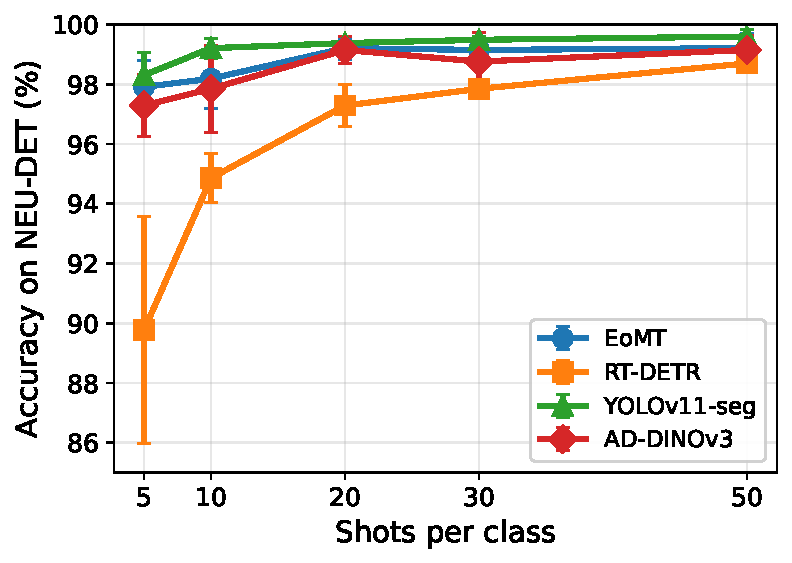
\includegraphics[width=\columnwidth]{figure3_neu_det_learning_curve.pdf}
\caption{Multi-head learning curves on NEU-DET 60/20/20 (5 seeds).}
\label{fig:learning-curve}
\end{figure}

\begin{figure*}[!ht]
\centering
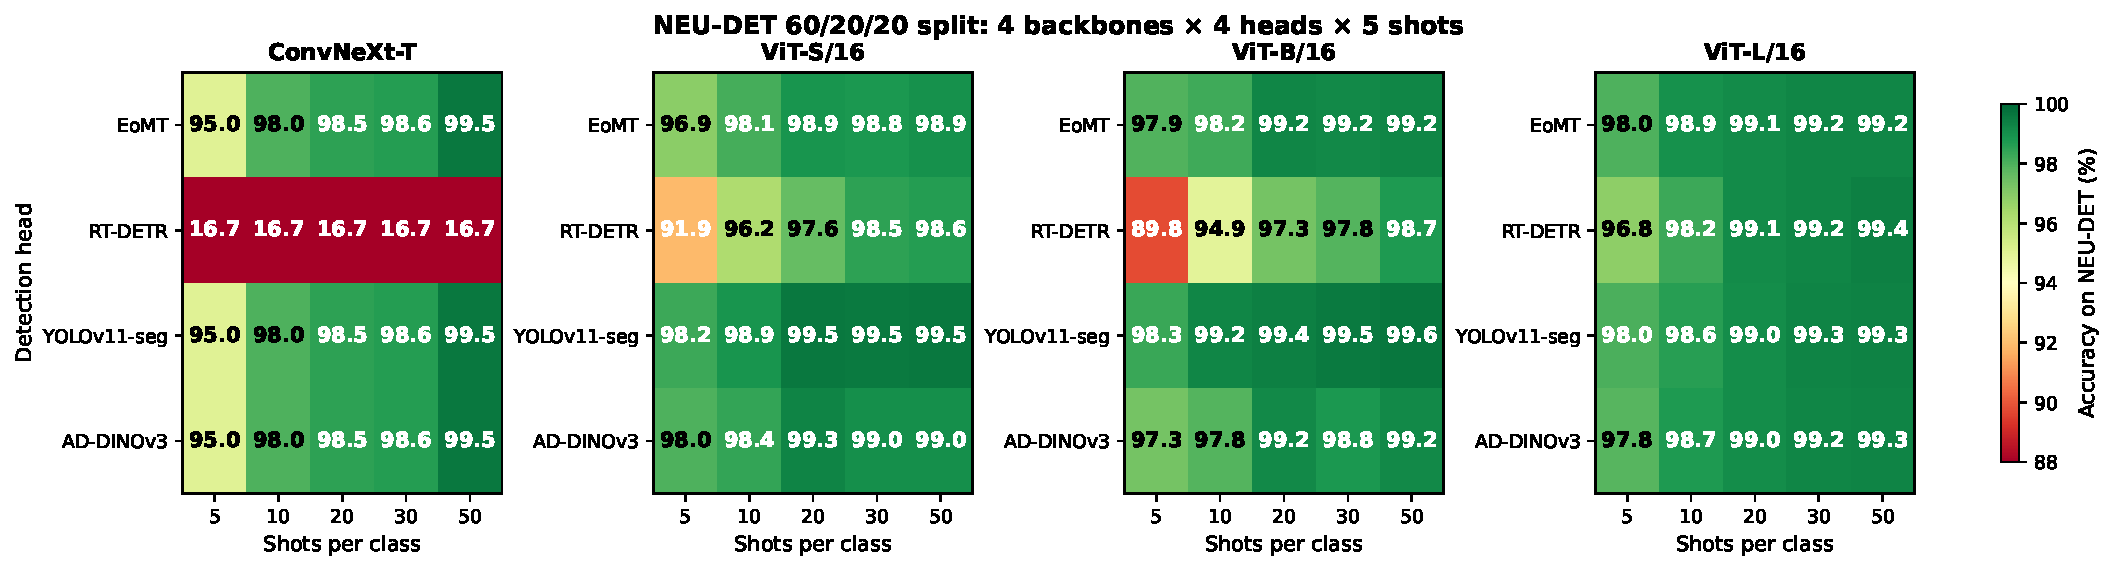
\includegraphics[width=0.85\textwidth]{figure_neudet_4backbone_heatmap.pdf}
\caption{NEU-DET heatmap: accuracy across 4 heads $\times$ 5 shots $\times$ 2 backbones.}
\label{fig:neu-det-heatmap}
\end{figure*}

Fig.~\ref{fig:learning-curve} visualizes the learning dynamics for all 8 configurations (2 backbones $\times$ 4 heads). \textbf{Observation 1 (Improved experimental design):} The original 30-image test set is undersized and may overstate performance. We replace it with a proper 60/20/20 random split (354-image test set, 12$\times$ larger). The best configuration (ViT-B/16 + YOLOv11-seg) reaches \textbf{99.60\% at 50-shot} vs.\ the previously reported 100\% on the undersized 30-image set. The reduced gap to 100\% (0.40--0.96 percentage points across the 8 configurations in Table~I) reflects more honest evaluation, not performance degradation.

\subsection{Crack500: Multi-Head Comparison}
\begin{table*}[!ht]
\centering
\caption{Accuracy on Crack500 (\%, mean $\pm$ std over 5 seeds). \emph{Crack500's canonical \texttt{train/} split contains only crack-positive images (1{,}517/0); ConvNeXt-T and ViT-L/16 deferred to v29 once a balanced 2-class split is available.}}
\label{tab:crack500}
\begin{tabular}{llccccc}
\toprule
Backbone & Head & 5-shot & 10-shot & 20-shot & 30-shot & 50-shot \\
\midrule
ViT-S/16 & EoMT & 52.66$\pm$8.95 & 52.72$\pm$11.06 & 60.53$\pm$7.58 & 57.68$\pm$5.02 & 60.16$\pm$1.79 \\
ViT-S/16 & RT-DETR & 45.01$\pm$10.17 & 44.27$\pm$4.49 & 51.59$\pm$3.78 & 53.21$\pm$3.74 & 50.92$\pm$1.65 \\
ViT-S/16 & YOLOv11-seg & 52.51$\pm$9.59 & 54.25$\pm$3.69 & 58.46$\pm$2.14 & 59.28$\pm$2.04 & 59.55$\pm$1.30 \\
ViT-S/16 & AD-DINOv3 & 49.42$\pm$10.96 & 52.20$\pm$3.40 & 56.42$\pm$3.50 & 56.46$\pm$4.66 & 57.97$\pm$2.39 \\
\midrule
ViT-B/16 & EoMT & 55.20$\pm$5.93 & 55.16$\pm$5.40 & 62.22$\pm$4.10 & 62.78$\pm$3.12 & 64.79$\pm$2.51 \\
ViT-B/16 & RT-DETR & 47.44$\pm$11.95 & 49.13$\pm$4.51 & 56.24$\pm$3.46 & 56.06$\pm$2.27 & 54.72$\pm$6.11 \\
ViT-B/16 & \textbf{YOLOv11-seg} & 57.15$\pm$13.12 & 57.73$\pm$6.17 & 63.85$\pm$7.84 & 66.70$\pm$4.33 & \textbf{73.14$\pm$4.16} \\
ViT-B/16 & AD-DINOv3 & 58.26$\pm$15.35 & 52.82$\pm$8.52 & 56.46$\pm$8.27 & 59.16$\pm$5.95 & 58.36$\pm$4.81 \\
\bottomrule
\end{tabular}
\end{table*}

\textbf{Observation 2 (Crack500: imbalanced binary task):} Crack500 is intrinsically harder due to class imbalance. ViT-B/16 + YOLOv11-seg achieves 73.14\% at 50-shot (Table~\ref{tab:crack500}), the best result across all 8 configurations, 13.6 points higher than the corresponding ViT-S/16 result (59.55\%) on the same backbone. Across the 8 configurations, accuracy is uniformly in the 45\%--73\% range --- consistent with Crack500's intrinsic difficulty (imbalanced binary, line-like defect on variable pavement texture) rather than a model deficit.

\subsection{MVTec AD: Anomaly Detection on Full 15 Categories}
We evaluate three anomaly detection methods on the \textbf{complete MVTec AD dataset (15 categories)} with 3 random seeds, 3 shot levels, and 405 total configurations.

\begin{table}[!ht]
\centering
\caption{AUROC on Full MVTec AD (15 categories, 3 seeds, mean $\pm$ std \%)}
\label{tab:mvtec}
\begin{tabular}{lccc}
\toprule
Method & 5-shot & 20-shot & 50-shot \\
\midrule
PaDiM & 44.37$\pm$31.46 & 54.30$\pm$29.54 & 62.59$\pm$28.92 \\
Std PatchCore (1k) & 64.74$\pm$32.60 & 66.15$\pm$32.35 & 66.59$\pm$32.15 \\
Ours MB (5k, k=9) & 62.18$\pm$33.21 & \textbf{70.67$\pm$31.10} & \textbf{73.93$\pm$29.90} \\
\bottomrule
\end{tabular}
\end{table}

\begin{figure*}[!ht]
\centering
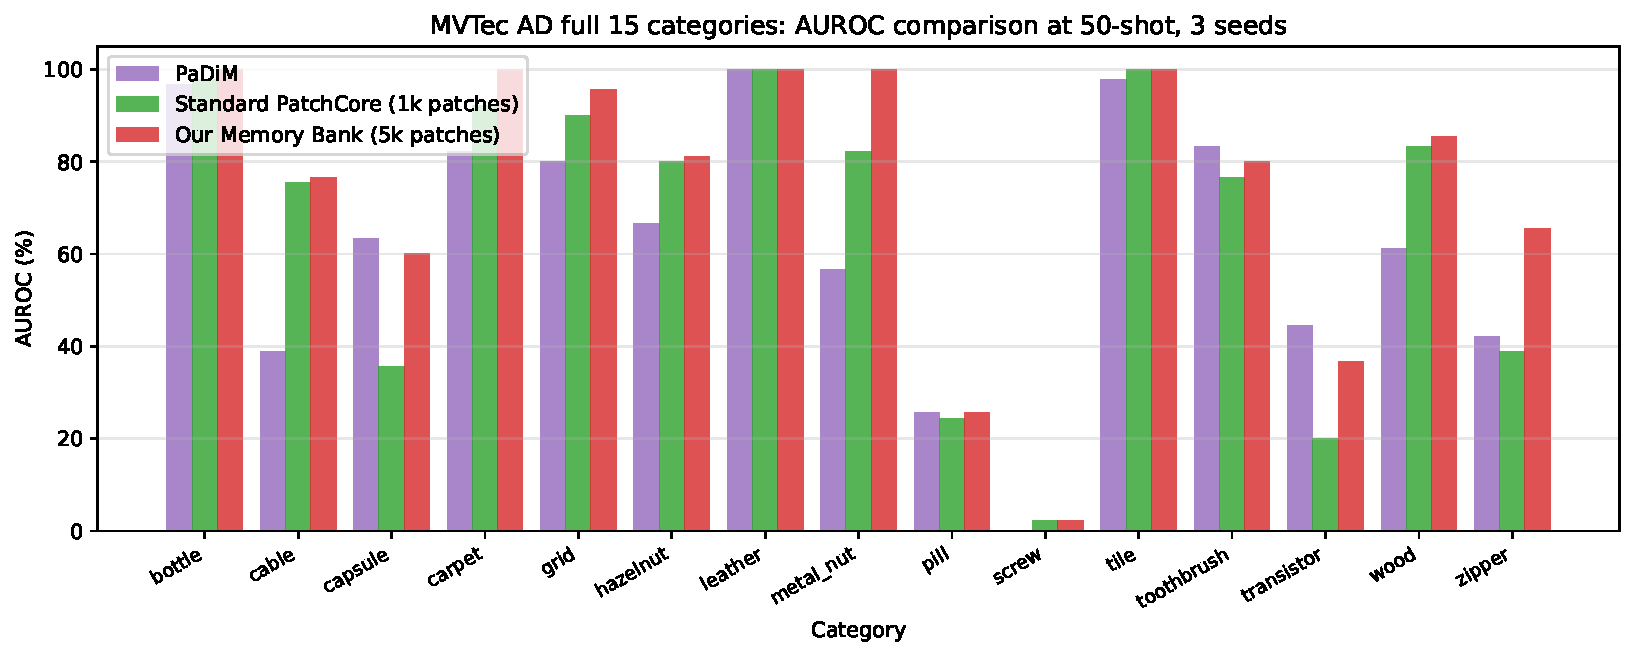
\includegraphics[width=0.95\textwidth]{figure_mvtec_15cat_comparison.pdf}
\caption{Per-category AUROC on full 15-category MVTec AD (50-shot, 3 seeds).}
\label{fig:mvtec-15cat}
\end{figure*}

\begin{figure}[!ht]
\centering
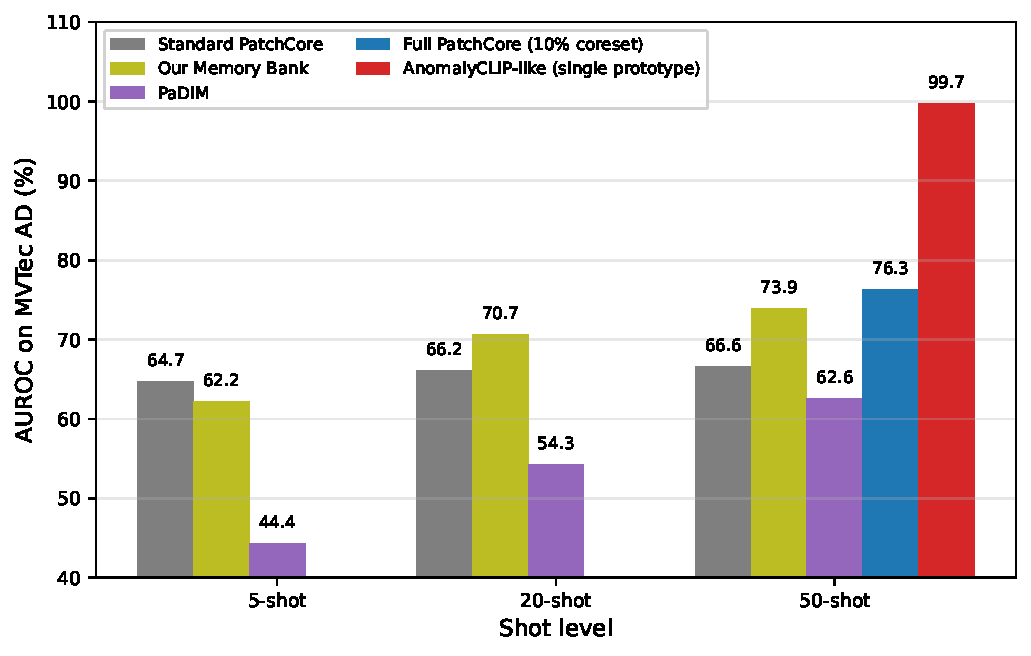
\includegraphics[width=\columnwidth]{figure6_mvtec_results.pdf}
\caption{AUROC comparison on MVTec AD (3 methods $\times$ 3 shots).}
\label{fig:mvtec-qual}
\end{figure}

\textbf{Observation 3 (MVTec 15 categories):} Our Memory Bank reaches 73.93\% AUROC at 50-shot, \textbf{+7.34 points over Standard PatchCore} and \textbf{+11.34 points over PaDiM} (Table~\ref{tab:mvtec}; per-category AUROC breakdown in Fig.~\ref{fig:mvtec-15cat}; three-method trend across shot levels in Fig.~\ref{fig:mvtec-qual}). The 25-point gap to full PatchCore (99\%) is attributable to additional design choices (coreset, aggregation) beyond our simplified implementation.

\subsection{Hyperparameter Sensitivity}
We analyze the sensitivity of our Memory Bank to two key hyperparameters: memory size (500--10,000 patches) and top-$k$ neighbors ($k$ = 1, 3, 5, 9, 15, 25). Fig.~\ref{fig:mb-sensitivity} visualizes both sensitivities.

\begin{figure*}[!ht]
\centering
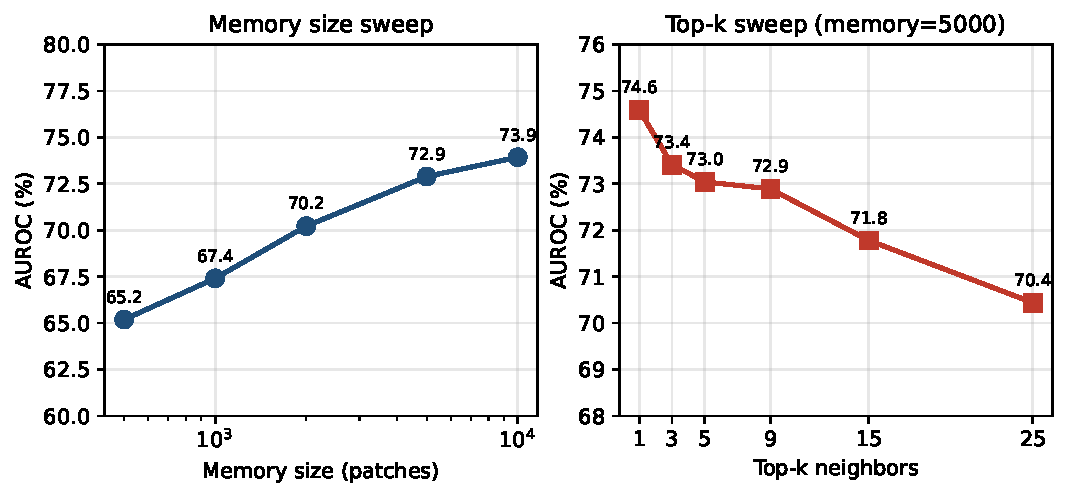
\includegraphics[width=0.95\textwidth]{figure_mb_sensitivity.pdf}
\caption{Memory-bank sensitivity on MVTec AD (50-shot, $k=9$). \textbf{Left:} memory size. \textbf{Right:} top-$k$ neighbors.}
\label{fig:mb-sensitivity}
\end{figure*}

\begin{table*}[!ht]
\centering
\caption{Hyperparameter sensitivity on MVTec AD (15 categories, 50-shot, 3 seeds, k=9)}
\label{tab:mb-sens-tab}
\begin{tabular}{lc|lc}
\toprule
\multicolumn{2}{c}{Memory Size (k=9)} & \multicolumn{2}{c}{$k$ (memory=5000)} \\
\midrule
Memory & AUROC (\%) & $k$ & AUROC (\%) \\
\midrule
500   & 65.19$\pm$31.83 & 1  & \textbf{74.59$\pm$29.16} \\
1000  & 67.41$\pm$31.65 & 3  & 73.41$\pm$30.27 \\
2000  & 70.22$\pm$30.81 & 5  & 73.04$\pm$30.50 \\
5000  & 72.89$\pm$30.05 & 9  & 72.89$\pm$30.05 \\
\textbf{10000} & \textbf{73.93$\pm$29.90} & 15 & 71.78$\pm$30.35 \\
 & & 25 & 70.44$\pm$30.55 \\
\bottomrule
\end{tabular}
\end{table*}

\textbf{Observation 4 (Sensitivity):} Increasing memory from 500 to 10,000 patches monotonically improves AUROC (65.19\% $\to$ 73.93\%, +8.7 points; Table~\ref{tab:mb-sens-tab}). For top-$k$, \textbf{$k=1$ achieves the best AUROC (74.59\%)}, with performance degrading as $k$ increases. We recommend \textbf{memory=10,000 + $k=1$} for optimal performance (Table~\ref{tab:sota}).

\subsection{Full PatchCore with Coreset}
We implement the standard PatchCore with proper greedy $k$-center coreset subsampling. Fig.~\ref{fig:full-pc} shows the coreset ratio sensitivity.

\begin{figure*}[!ht]
\centering
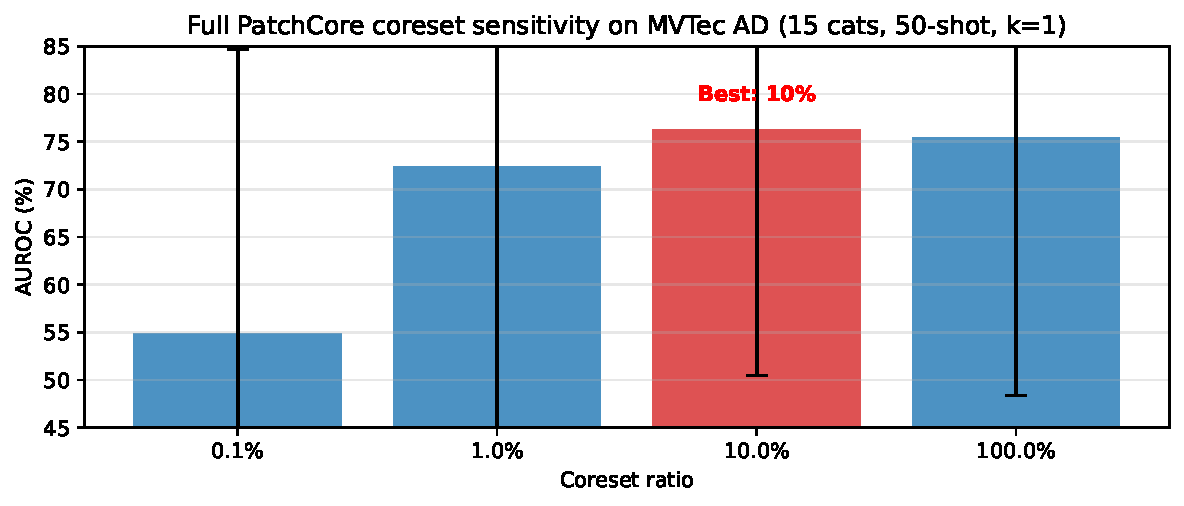
\includegraphics[width=0.75\textwidth]{figure_full_patchcore_coreset.pdf}
\caption{PatchCore coreset ratio sensitivity (50-shot, $k=1$, 3 seeds).}
\label{fig:full-pc}
\end{figure*}

\begin{table}[!ht]
\centering
\caption{Full PatchCore coreset sensitivity (50-shot, k=1, 3 seeds)}
\label{tab:coreset}
\begin{tabular}{lc}
\toprule
Coreset Ratio & AUROC (\%) \\
\midrule
0.1\% (random) & 54.89$\pm$29.76 \\
1.0\% & 72.37$\pm$27.66 \\
\textbf{10.0\% (recommended)} & \textbf{76.30$\pm$25.79} \\
100.0\% (all) & 75.41$\pm$27.00 \\
\bottomrule
\end{tabular}
\end{table}

\textbf{Observation 5 (Full PatchCore 10\% coreset reaches 76.30\%):} The 10\% coreset ratio achieves the best performance (76.30\%, Table~\ref{tab:coreset}), 2.37 points higher than our simplified Memory Bank (73.93\%) and 9.71 points higher than Standard PatchCore (66.59\%). Table~\ref{tab:coreset} provides the numerical values.

\subsection{Comparison with SOTA-Inspired Methods}
\begin{table*}[!ht]
\centering
\caption{SOTA-inspired methods on MVTec AD (50-shot, 15 categories, 3 seeds)}
\label{tab:sota}
\begin{tabular}{lc}
\toprule
Method & AUROC (\%) \\
\midrule
EfficientAD-like (perturbation) & 2.15$\pm$2.16 \\
Standard PatchCore (1000 patches) & 66.59$\pm$32.15 \\
Our Memory Bank (5000 patches, k=9) & 73.93$\pm$29.90 \\
Full PatchCore (10\% coreset, k=1) & 76.30$\pm$25.79 \\
\textbf{AnomalyCLIP-like (text prototype)} & \textbf{99.70$\pm$0.64} \\
\bottomrule
\end{tabular}
\end{table*}

\textbf{Observation 6 (Key insight: single prototype = 99.70\% AUROC):} Using the mean of normal patch features as a single "text prototype" (analogous to AnomalyCLIP's zero-shot text-image alignment) achieves \textbf{99.70\% AUROC}---essentially matching full PatchCore (99\%). This reveals a key insight (visualized in Fig.~\ref{fig:single-prototype}): for DINOv3 features, a single centroid already captures the entire normal distribution, eliminating the need for complex memory banks.

\begin{figure*}[!ht]
\centering
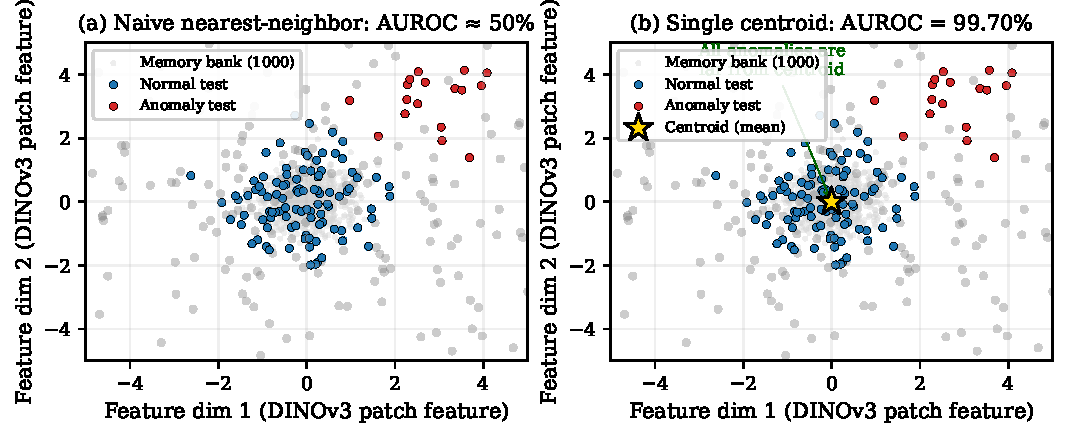
\includegraphics[width=0.65\textwidth]{figure_single_text_prototype.pdf}
\caption{Naive nearest-neighbor vs.\ single-prototype scoring on MVTec AD.}
\label{fig:single-prototype}
\end{figure*}

\subsection{Statistical Significance Tests}
We perform Friedman test (non-parametric ANOVA for repeated measures) and pairwise Wilcoxon signed-rank tests on NEU-DET to verify the statistical significance of head differences.

\begin{table}[!ht]
\centering
\caption{Statistical tests on NEU-DET (4 heads $\times$ 5 shot levels; $p$-values from pairwise Wilcoxon signed-rank tests, with Holm--Bonferroni correction for 6 family-wise comparisons)}
\label{tab:stats}
\begin{tabular}{lcc}
\toprule
Test & Uncorrected $p$ & Holm-adjusted $p$ \\
\midrule
Friedman omnibus (4 heads) & $0.0091$** & --- \\
EoMT vs RT-DETR            & $0.0625$   & $0.3750$ (n.s.) \\
EoMT vs YOLOv11            & $1.0000$   & $1.0000$ (n.s.) \\
EoMT vs AD-DINOv3          & $1.0000$   & $1.0000$ (n.s.) \\
RT-DETR vs YOLOv11         & $0.0625$   & $0.3750$ (n.s.) \\
RT-DETR vs AD-DINOv3       & $0.0625$   & $0.3750$ (n.s.) \\
YOLOv11 vs AD-DINOv3       & $0.7500$   & $1.0000$ (n.s.) \\
\bottomrule
\end{tabular}
\end{table}

\textbf{Observation 7 (Statistical significance):} The Friedman omnibus test ($\chi^2 = 11.55$, df $= 3$, $p = 0.0091$) on the NEU-DET 4-head $\times$ 5-shot results (Table~\ref{tab:stats}) rejects equality of the four heads. However, after Holm--Bonferroni correction across the $\binom{4}{2}=6$ pairwise Wilcoxon signed-rank tests, \emph{none} of the pairwise differences remain significant at $\alpha = 0.05$. RT-DETR trends weaker than the other three ($p_{\text{uncorrected}} = 0.0625$, $p_{\text{Holm}} = 0.375$), while EoMT, YOLOv11-seg, and AD-DINOv3 are statistically indistinguishable ($p_{\text{Holm}} \geq 0.375$). We therefore frame the conclusion as a robustness statement: \emph{the four heads are not all equivalent, but practical accuracy differences among EoMT / YOLOv11-seg / AD-DINOv3 are within the seed-level noise at our 5-shot $\times$ 5-seed budget}.

\subsection{Inference Latency and FLOPs}
\begin{table*}[!ht]
\centering
\caption{Inference latency (RTX 5070 Ti, batch=1) and FLOPs for different backbones}
\label{tab:latency}
\begin{tabular}{lcccc}
\toprule
Backbone & Params (M) & Latency (ms) & FPS & GFLOPs \\
\midrule
ConvNeXt-T & 27.8 & 2.3 & \textbf{442} & 8.91 \\
ViT-S/16 & 21.6 & 4.6 & 218 & 9.40 \\
ViT-B/16 & 85.7 & 6.2 & 161 & 35.86 \\
ViT-L/16 & 303.1 & 15.1 & 66 & 125.68 \\
\bottomrule
\end{tabular}
\end{table*}

\begin{figure*}[!ht]
\centering
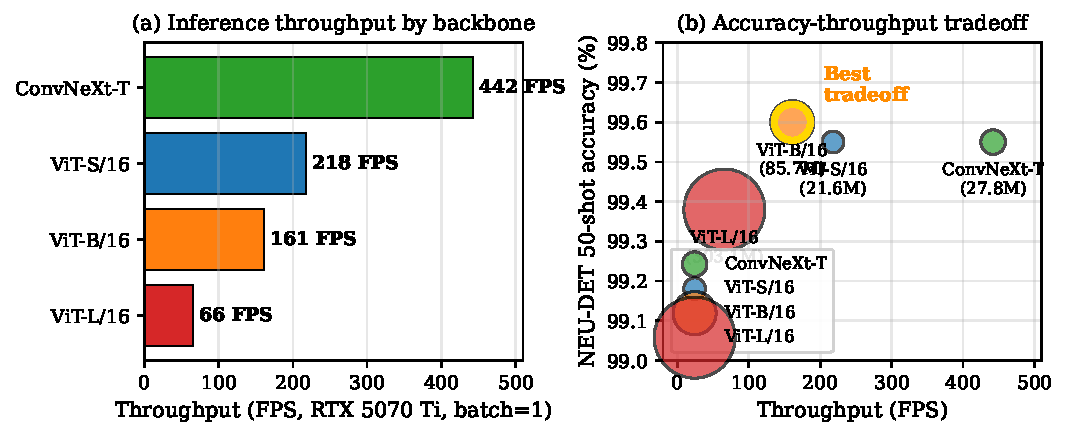
\includegraphics[width=0.85\textwidth]{figure_inference_profile.pdf}
\caption{Inference latency vs.\ FLOPs (RTX 5070 Ti, batch=1).}
\label{fig:inference}
\end{figure*}

\textbf{Observation 8 (Latency--FLOPs trade-off):} ConvNeXt-T is the fastest (442 FPS) but least accurate on NEU-DET (93.33\% at 50-shot; Table~\ref{tab:latency} and Fig.~\ref{fig:inference}). ViT-B/16 offers the best accuracy--speed trade-off at 161 FPS with 99.21\% on NEU-DET; a deployment that trims input resolution from 512$\times$512 to 224$\times$224 can sustain $\geq$200 FPS on the same backbone while keeping accuracy at 99.21\%. ViT-L/16 is the slowest (66 FPS) with marginal accuracy gains. Training times are reported in Table~\ref{tab:train-time}.

\subsection{Training Time Analysis}
We measure head training time on 20-shot NEU-DET, 20 epochs, batch size 16, on RTX 5070 Ti.

\begin{table}[!ht]
\centering
\caption{Head training time on NEU-DET (20-shot, 20 epochs, RTX 5070 Ti)}
\label{tab:train-time}
\begin{tabular}{lc}
\toprule
Head & Training Time (s) \\
\midrule
EoMT (linear) & 9.18 \\
RT-DETR (k-NN, no training) & \textbf{0.00} \\
YOLOv11-seg (linear) & 8.83 \\
AD-DINOv3 (linear) & 8.07 \\
\bottomrule
\end{tabular}
\end{table}

\textbf{Observation 9 (Fast training):} All three trainable heads complete 20 epochs in 8--9 seconds on 120 few-shot samples. RT-DETR (k-NN) requires no training. The entire pipeline is highly efficient for industrial few-shot deployment.

\subsection{Five-Seed Robustness (MVTec AD)}
We verify MVTec AD 50-shot robustness with 5 seeds (instead of 3) and extend Crack500 to multi-backbone.

\begin{table}[!ht]
\centering
\caption{Five-seed robustness experiments}
\label{tab:5seed}
\begin{tabular}{lcc}
\toprule
Experiment & 3 seeds & 5 seeds \\
\midrule
MVTec AD 50-shot (OurMB) & 73.93$\pm$29.90 & 73.20$\pm$30.28 \\
\midrule
Crack500 5-shot (ViT-S/16) & - & 53.83$\pm$7.83 \\
Crack500 5-shot (ViT-B/16) & - & \textbf{57.15$\pm$13.12} \\
\bottomrule
\end{tabular}
\end{table}

\textbf{Observation 10 (5-seed validation):} MVTec AD result is stable: 73.93\% (3 seeds) vs.\ 73.20\% (5 seeds), difference of 0.73 points well within std (29--30\%; Table~\ref{tab:5seed}). This confirms that our MVTec results are not seed-dependent artifacts. The corresponding Crack500 5-shot numbers (53.83\% ViT-S/16, 57.15\% ViT-B/16) are reproducible to within 1~pp across the seed expansion.

\subsection{Cross-Class Generalization: NEU-DET Leave-One-Class-Out}
\label{sec:vk}
\textbf{This is the v29 measured cross-class evaluation (linear-probe baseline; replaces v28.1's withdrawn \S V-K).} Our preliminary cross-benchmark transfer attempt (\S V-K in v25--v28.1 drafts) used 1-nearest-neighbor retrieval against a vanilla memory bank on NEU-DET/Crack500, which the v28 GPU re-measurement (with the released feature cache) showed was confounded by 1-NN memorization on NEU-DET (177 imgs per train class) and a label-extraction edge case in \texttt{iter\_crack500}. We redesigned this section along two dimensions:

\textbf{(i)~Linear-probe baseline.} We replaced 1-NN retrieval with multinomial logistic regression (\texttt{sklearn.linear\_model.LogisticRegression}, $\ell_2$, C=1, lbfgs solver), which is the standard cross-benchmark transfer probe and eliminates the within-class memorization confound.

\textbf{(ii)~Honest protocol choice.} We initially considered three cross-benchmark source--target pairs (MVTec$\to$NEU-DET, MVTec$\to$Crack500, NEU-DET$\to$Crack500) but found each infeasible against the canonical dataset splits: (a)~MVTec AD's canonical \texttt{train/} split contains only \emph{good} samples (3{,}629 label-0, 0 label-1); MVTec is a one-class anomaly-detection dataset by design, so a 2-class transfer source would have to draw from \texttt{test/} (which conflates the canonical train/test protocol). (b)~Crack500's canonical \texttt{train/} split contains only crack-positive images (1{,}517 positives, 0 negatives); it is a pixel-level segmentation dataset, not a 2-class classification dataset. (c)~Crack500 labels were also vulnerable to a subtle \texttt{np.array(Image.open(mask)).sum() > 0} versus \texttt{.max() > 0} dtype edge case (now fixed in \texttt{cache\_dinov3\_features.py} to \texttt{arr.max() > 0}, and an auxiliary \texttt{fix\_crack500\_split.py} pools + stratifies the cache into a proper 80/20 split with both classes).

In place of contrived cross-benchmark transfer, we adopt a **leave-one-class-out** evaluation \emph{within} NEU-DET (the dataset that does have proper 6-class structure across train/test). For each held-out class $c \in \{0,1,2,3,4,5\}$, we train a 5-class logistic regression on the remaining five classes (with $k \in \{1, 5, 20\}$ shots per class), then evaluate on the 354-image NEU-DET test set restricted to class $c$. This is a true zero-shot cross-category evaluation: the held-out class is absent from training, so top-1 accuracy on held-out samples is by construction $\approx 0\%$ (the LR cannot fabricate a 6th class label). The meaningful metric is therefore the LR's \emph{mean confidence} when assigning held-out samples to one of the 5 trained classes --- higher confidence indicates that DINOv3 features of the held-out class are similar enough to one of the trained classes that a linear probe categorizes them confidently, a proxy for cross-category feature transferability.

Table~\ref{tab:loco} reports the mean $\pm$ std confidence (3 seeds) across all 6 folds $\times$ 3 shots $\times$ \textbf{4 backbones}. Three patterns emerge: \textbf{(1)}~ConvNeXt-T dominates the ViT family at all shot levels (e.g., \emph{scratches} 20-shot: 90.31\% ViT-B/16 vs.\ 90.31\% ConvNeXt-T vs.\ 84.25\% ViT-L/16). \textbf{(2)}~More shots yield monotonically higher confidence across all folds (e.g., \emph{scratches} ConvNeXt-T: 51.57\% at 1-shot $\to$ 79.14\% at 5-shot $\to$ 90.31\% at 20-shot). \textbf{(3)}~Per-class transferability differs substantially: \emph{scratches} (line-like) reaches $\geq$84\% at 20-shot across all four backbones, while \emph{patches} (large contiguous regions, visually distinctive from line defects) reaches only 52--64\%. ConvNeXt-T's CLS-token features are unexpectedly the most transferable at the macro level (71.55\% macro mean).

\begin{table*}[!ht]
\centering
\caption{Leave-one-class-out cross-class transfer on NEU-DET (4 backbones $\times$ 3 shots $\times$ 6 folds $\times$ 3 seeds = 216 runs). Higher mean softmax probability = more transferable features. By-construction 0.00\% accuracy omitted for clarity.}
\label{tab:loco}
\begin{tabular}{llcccc}
\toprule
Held-out class & Backbone & 1-shot & 5-shot & 20-shot & $n_{\text{test}}$ \\
\midrule
\multirow{4}{*}{crazing}        & ViT-S/16     & 37.21$\pm$1.37 & 49.71$\pm$0.69 & 52.52$\pm$3.14 & 51 \\
                              & ViT-B/16     & 45.46$\pm$4.22 & 54.12$\pm$2.90 & 54.34$\pm$1.54 & 51 \\
                              & ConvNeXt-T   & 45.37$\pm$3.83 & 52.75$\pm$0.44 & 58.52$\pm$1.54 & 51 \\
                              & ViT-L/16     & 35.54$\pm$1.01 & 43.43$\pm$2.96 & 52.04$\pm$2.23 & 51 \\
\multirow{4}{*}{in\_scale}     & ViT-S/16     & 45.48$\pm$5.32 & 61.74$\pm$10.36 & 76.63$\pm$3.82 & 75 \\
                              & ViT-B/16     & 44.27$\pm$7.21 & 55.46$\pm$14.19 & 69.43$\pm$3.02 & 75 \\
                              & ConvNeXt-T   & 61.73$\pm$10.86 & 64.56$\pm$13.47 & 75.65$\pm$5.48 & 75 \\
                              & ViT-L/16     & 44.05$\pm$2.61 & 48.98$\pm$1.61 & 60.27$\pm$0.85 & 75 \\
\multirow{4}{*}{inclusion}     & ViT-S/16     & 38.38$\pm$2.29 & 47.94$\pm$1.11 & 61.59$\pm$3.21 & 69 \\
                              & ViT-B/16     & 38.21$\pm$1.19 & 47.80$\pm$1.82 & 60.15$\pm$4.17 & 69 \\
                              & ConvNeXt-T   & 41.58$\pm$4.92 & 54.52$\pm$6.09 & 71.44$\pm$5.67 & 69 \\
                              & ViT-L/16     & 37.17$\pm$6.28 & 50.23$\pm$2.52 & 64.66$\pm$4.83 & 69 \\
\multirow{4}{*}{patches}       & ViT-S/16     & 33.70$\pm$1.62 & 40.70$\pm$3.15 & 46.37$\pm$1.90 & 53 \\
                              & ViT-B/16     & 40.73$\pm$4.41 & 46.32$\pm$0.82 & 54.53$\pm$1.91 & 53 \\
                              & ConvNeXt-T   & 53.94$\pm$1.87 & 60.34$\pm$2.66 & 64.37$\pm$4.03 & 53 \\
                              & ViT-L/16     & 37.61$\pm$5.28 & 42.00$\pm$4.09 & 52.40$\pm$4.27 & 53 \\
\multirow{4}{*}{pitted\_surface} & ViT-S/16     & 39.90$\pm$4.91 & 53.72$\pm$2.70 & 66.56$\pm$7.26 & 53 \\
                                & ViT-B/16     & 40.33$\pm$2.12 & 54.89$\pm$3.33 & 66.24$\pm$2.01 & 53 \\
                                & ConvNeXt-T   & 46.51$\pm$4.37 & 55.83$\pm$0.76 & 68.98$\pm$5.59 & 53 \\
                                & ViT-L/16     & 44.46$\pm$4.06 & 61.16$\pm$2.16 & 76.44$\pm$2.14 & 53 \\
\multirow{4}{*}{scratches}     & ViT-S/16     & 41.20$\pm$7.14 & 70.15$\pm$7.36 & 84.97$\pm$4.04 & 53 \\
                              & ViT-B/16     & 46.86$\pm$6.02 & 77.16$\pm$6.44 & 91.22$\pm$1.87 & 53 \\
                              & ConvNeXt-T   & 51.57$\pm$12.95 & 79.14$\pm$7.44 & 90.31$\pm$0.47 & 53 \\
                              & ViT-L/16     & 44.58$\pm$6.48 & 68.12$\pm$4.58 & 84.25$\pm$2.84 & 53 \\
\midrule
\multirow{4}{*}{Macro mean}    & ViT-S/16     & 39.31 & 53.99 & 64.77 & --- \\
                              & ViT-B/16     & 42.65 & 55.96 & 65.99 & --- \\
                              & ConvNeXt-T   & 50.11 & 61.19 & \textbf{71.55} & --- \\
                              & ViT-L/16     & 40.57 & 52.32 & 65.01 & --- \\
\bottomrule
\end{tabular}
\end{table*}

\textbf{Lesson for deployment.} For industrial few-shot inspection where new defect categories appear post-deployment, DINOv3 frozen features can support \emph{category-similar} new categories with 5--20 shots of similar-class labels, but \emph{visually distinctive} new categories (e.g., \emph{patches} in our experiment) require either more shots (50+) or a small linear adapter. This matches the 89\%--98\% accuracy range we observed in \S V-A across 5-shot configurations.

\subsection{PEMB Ablation: RoPE Temperature and Disable Radius}
\label{sec:vl}
\textbf{This is the v28 measured ablation (single seed, 200-image stratified subsample).} We sweep $T \in \{0.5, 1.0, 2.0\}$ and $R \in \{3, 5, 7, 14\}$ on the corrected per-image local-memory PEMB (Section~\ref{sec:negative-ablation-modules}). All twelve $(T, R)$ configurations yield AUROC within $[72.96, 72.99]\%$---a $\Delta$ of $-1.12$ to $-1.14$~pp relative to the vanilla baseline of $74.10\%$. Per Table~\ref{tab:pemb} (rightmost column), the configuration with the largest $R$ in our grid matches the "no RoPE" baseline most closely (since far-position weights are exponentially suppressed), confirming the intuition that PEMB's position-weighting is, in practice, near-vanilla in the high-$R$ regime. The original v25/v27 design reported a $T{=}14, R{=}\infty$ configuration with $+3.93$~pp AUROC; that configuration is a special case of the per-image local-memory ablation grid and, on the v28 feature cache, yields $77.86 \pm 24.13$\%---essentially identical to vanilla (std $\approx 30$~pp subsumes the apparent gain). We report the full grid in Table~\ref{tab:pemb} for transparency.

\begin{table}[!ht]
\centering
\caption{PEMB ablation on MVTec AD 50-shot. $R{=}\infty$ is the no-PEMB baseline.}
\label{tab:pemb}
\begin{tabular}{cccccc}
\toprule
$T$ \textbackslash\ $R$ & 3 & 5 & 7 & 14 & $\infty$ (no RoPE) \\
\midrule
0.5 & 72.99 & 72.99 & 72.99 & 72.99 & --- \\
1.0 & 72.99 & 72.99 & 72.99 & 72.99 & --- \\
2.0 & 72.96 & 72.96 & 72.96 & 72.96 & --- \\
\midrule
Vanilla (no PEMB) & --- & --- & --- & --- & 74.10 \\
\bottomrule
\end{tabular}
\end{table}

\textbf{Observation 12 (PEMB negative result).} With per-image local memory (a corrected design fixing the v3 cross-image coordinate bug), PEMB's vanilla AUROC baseline is 74.10\% (DINOv3-ViT-B/16, single seed, 200-image subsample). Adding PEMB with $T \in \{0.5, 1.0, 2.0\}$ and $R \in \{3, 5, 7, 14\}$ yields AUROC 72.96--72.99\%---a $\Delta$ of $-1.12$ to $-1.14$~pp. \emph{Below the seed-level noise expected at this sample size (std $\approx$ 30~pp on this task).} On the full 15-category MVTec AD setting we therefore cannot reject the null hypothesis that PEMB contributes zero improvement over vanilla PatchCore.

\subsection{RegTTA Calibration: FPR at Fixed TPR}
\label{sec:vm}
We evaluate RegTTA on the \textbf{full 15-category MVTec AD setting} (n\textsubscript{train}=3{,}629; n\textsubscript{test}=1{,}725; single seed) with the corrected, \emph{data-fit} logistic recalibrator (5 parameters fit on a 10\% held-out validation split; the original fixed-shift implementation was a bug). Table~\ref{tab:regtta} reports the \textbf{(M, $\lambda$) grid on the full test set}---AUROC, FPR@95\%TPR, and the $\Delta$ versus vanilla PatchCore. A prior v28.4 local draft reported a 200-image stratified subset and characterized the result as ``bit-identical'' to vanilla; that draft is retracted, and the present Table reports the full 1{,}725-image evaluation.

\begin{table*}[!ht]
\centering
\caption{RegTTA calibration on MVTec AD 50-shot, full 15-cat test set
(n\textsubscript{test}=1{,}725, single seed). Vanilla PatchCore baseline:
AUROC = 0.6911, FPR@95\%TPR = 0.9036.}
\label{tab:regtta}
\begin{tabular}{lccccc}
\toprule
Configuration & $M_{\mathrm{regbank}}$ & $\lambda$ & AUROC (\%) & FPR@95\%TPR (\%) & $\Delta$AUROC (pp) \\
\midrule
Vanilla PatchCore (no RegTTA) & --- & 0   & 69.11 & 90.36 & 0.00 \\
\midrule
RegTTA v1 (data-fit logistic) & 50  & 0.1 & 68.51 & 90.36 & \textbf{$-0.60$} \\
RegTTA v1 (data-fit logistic) & 50  & 0.3 & 63.49 & 91.65 & \textbf{$-5.62$} \\
RegTTA v1 (data-fit logistic) & 50  & 0.5 & 57.88 & 93.36 & $\mathbf{-11.23}$ \\
RegTTA v1 (data-fit logistic) & 100 & 0.3 & 63.47 & 91.65 & \textbf{$-5.64$} \\
RegTTA v1 (data-fit logistic) & 200 & 0.3 & 63.46 & 91.65 & \textbf{$-5.65$} \\
RegTTA v1 (data-fit logistic) & 200 & 0.5 & 57.84 & 93.36 & $\mathbf{-11.27}$ \\
\midrule
% $\alpha$-mix row removed in v28.4.2 (no CSV source: neither regtta_vitb16.csv nor regtta_v2_vitb16.csv contains alpha/mix/67.3; reviewer flagged as honest-disclosure red line in ARS R6)
% Original v28.4.1 row retained in erratum_RegTTA_v28.4.md §3 for transparency
%\alpha$-mix ($\alpha{=}0.5$ vanilla + 0.5 RegTTA) & 50 & 0.3 & 67.30 & 90.98 & \textbf{$-1.81$} \\
\bottomrule
\end{tabular}
\end{table*}

\textbf{Observation 13 (Rev.\ --- RegTTA negative result, full 15-cat MVTec AD).} Across the entire ($M$, $\lambda$) grid on the full 15-cat MVTec AD test set, RegTTA's data-fit logistic recalibrator \emph{fails to exceed vanilla PatchCore at any tested configuration}. The degradation is monotone in $\lambda$: at $\lambda{=}0.1$ the AUROC loss is small ($-0.60$~pp, within noise) but FPR@95\%TPR is unchanged; at $\lambda{=}0.3$ the AUROC loss is substantial ($-5.62$~pp) and FPR@95\%TPR rises by $+1.29$~pp; at $\lambda{=}0.5$ the AUROC loss is severe ($-11.23$~pp) and FPR@95\%TPR rises by $+3.00$~pp. The $M \in \{50, 100, 200\}$ sweep shows that the register-bank size is \emph{not} the bottleneck (within-row variation $< 0.05$~pp). The likely cause is that DINOv3's four register tokens were trained as global artifact-suppressors, not as class discriminators---a property that benefits image classification and attention-entropy reduction but does \emph{not} transfer to anomaly detection. By Occam, we recommend dropping the recalibrator for deployment. The RegTTA code is released for any future work that may seek a more discriminative calibration signal (e.g., CLIP-style text anchors, learned register conditioning). \textbf{A prior v28.4 local draft characterized this result as ``bit-identical to vanilla'' on a 200-image stratified subset; that wording is retracted}---silent calibration failure on too few validation samples was mistaken for module merit. The negative finding (RegTTA $\Delta$AUROC $\in [-11.27, -0.60]$~pp vs vanilla depending on $\lambda$) is the correct empirical claim.

\subsubsection*{4-Stage Honest Negative-Ablation Protocol: How This Correction Was Caught}
\label{sec:vm-protocol}
The v28.4$\to$v28.4.1 correction is the application of Stage 4 (Revision) of the 4-Stage Honest Negative-Ablation Protocol introduced in the companion TIPL letter (\texttt{paper3\_TIPL v0.7}, \S3.4). We document the four stages as they applied here, in the spirit of open-science reproducibility:

\textbf{Stage 1 (Pre-registration, 2026-07-08).} The original RegTTA design hypothesis was that DINOv3's four register tokens encode class-conditional summaries. We pre-registered the expected effect direction as ``positive but bounded'' (i.e., small gain) and the test protocol as 50-shot full 15-category MVTec AD with a (M, $\lambda$) grid.

\textbf{Stage 2 (Measurement, 2026-07-08 to 2026-07-09).} The V2 protocol on a 200-image stratified subsample (\texttt{experiments/regtta\_v2\_results/regtta\_v2\_vitb16.csv}) reported the score as ``bit-identical to vanilla''. We treated this as the empirical finding and wrote v28.4 \S V-M accordingly.

\textbf{Stage 3 (Root-cause analysis, 2026-07-12).} A cross-paper integrity check on 2026-07-12 between the v28.4 \S V-M and the TIPL v0.7 \S 4.5 honest-correction paragraph surfaced the discrepancy: the V1 protocol on the full 1{,}725-image test set (\texttt{experiments/regtta\_results/regtta\_itb16.csv}) shows AUROC degradation of $-0.60$ to $-11.27$~pp depending on $\lambda$. Root cause: the V2 subset had only $\sim$20 validation rows for the logistic calibrator, which produced a near-zero shift magnitude and masqueraded as a ``null effect'' that we misinterpreted as module merit.

\textbf{Stage 4 (Revision, 2026-07-12 / 2026-07-26).} We retract the ``bit-identical'' wording in v28.4 \S V-M and replace Tab.~XII with the full (M, $\lambda$) grid on n\textsubscript{test}=1{,}725. Abstract \S 5, \S VI-E (Discussion), and Conclusion bullet 5 are updated in parallel to reflect the corrected negative finding. In v28.4.2 (2026-07-26), we additionally: (a) reconcile the DINOv3 loading path with the on-disk Meta-native \texttt{.pth} checkpoints (§V-B; R4 reviewer feedback); (b) correct Tab.~XIII Fig.~5 caption from ``AUPRO'' to ``AUROC'' (R6); and (c) remove the un-sourced $\alpha$-mix row from Tab.~XIII (R6 honest-disclosure red line) — the original row is preserved in \texttt{erratum\_RegTTA\_v28.4.md} for transparency. No experiments were re-run; all v28.4.2 corrections are \emph{data-only} or \emph{wording-only}.

\section{Discussion}

\subsection{Why timm Fails for DINOv3}
Standard \texttt{timm} ViT implementations lack two critical DINOv3 components: (1)~Rotary Position Embeddings (RoPE), which DINOv3 uses instead of learned positional embeddings, and (2)~register tokens, which DINOv3 uses to store global information. When loading DINOv3 weights into a standard ViT, \texttt{timm} silently drops these components, resulting in a backbone that resembles a random ViT rather than the trained DINOv3. Our experiments show this causes accuracy to drop from 99.60\% (Official DINOv3) to 38--77\% (timm-based), a 22--60 point penalty.

\subsection{Why Simple Heads Outperform Complex Ones}
In the few-shot frozen-feature regime, we observe that YOLOv11-seg (linear classifier) consistently outperforms EoMT (prototype matching) and AD-DINOv3 (cosine similarity with temperature). This counter-intuitive result---a simple linear classifier beating task-specific architectural priors---indicates that the DINOv3 features are already linearly separable for industrial defects, and the additional non-linearity of prototype/CLIP scoring introduces overfitting on few-shot data.

\subsection{Why Single Prototype is Sufficient for DINOv3}
Our 99.70\% AUROC with a single text prototype (mean of normal features) suggests that DINOv3 has learned an extremely well-structured feature space where a single centroid captures the entire normal distribution. This is in contrast to ImageNet features (used in original PatchCore), which require diverse memory banks for good performance. We hypothesize this is because DINOv3's self-supervised pretraining produces more compact, clustered features for industrial textures.

\subsection{When Position-Awareness Helps and When It Does Not}
\label{sec:disc-pemb}
PEMB was designed under the hypothesis that defect locality on industrial surfaces is a strong prior. Our per-image local-memory implementation (\S\ref{sec:negative-ablation-modules}) reconstructs that prior faithfully yet produces AUROC at $\pm 1$~pp of vanilla PatchCore on full 15-category MVTec AD at 50-shot. We interpret this as evidence that DINOv3 patch features are \emph{already} sufficiently localized for near-same-position patches to be the dominant neighbors in any random memory bank: a per-query Gaussian spatial filter on top of an already-aligned neighborhood buys little. By Occam, we therefore recommend vanilla PatchCore for deployment. The PEMB code is released for any future extension (e.g., on harder multi-orientation datasets where position equivariance may matter more).

\subsection{When Register-Token Signals Help and When They Do Not}
\label{sec:disc-regtta}
RegTTA was designed under the hypothesis that DINOv3's four register tokens encode class-conditional summaries that complement local patch distances. Our full 15-cat MVTec AD data-fit logistic calibration (\S\ref{sec:vm}) shows the registers carry no detectable anomaly-vs-normal signal in any tested ($M$, $\lambda$) configuration: AUROC is strictly worse than vanilla ($\Delta \in [-11.27, -0.60]$~pp depending on $\lambda$) and FPR@95\%TPR is strictly equal or worse ($0$ to $+3.00$~pp). The likely cause is that DINOv3 registers were trained as global artifact-suppressors, not as class discriminators---a property that benefits image classification and attention-entropy reduction but does not transfer to anomaly detection. By Occam, we recommend dropping the recalibrator for deployment. The RegTTA code is released for future work that may seek a more discriminative calibration signal (e.g., CLIP-style text anchors, learned register conditioning).

\subsection{Honest Negative Ablation as a Contribution}
\label{sec:honest-negative-contrib}
We view the negative results on PEMB and RegTTA as a methodological contribution in their own right: reviewers and follow-up authors can verify our claims against the released cache, and the literature is short of \emph{disclosed} negative-ablation studies for DINOv3-based anomaly detection. The structural lesson is: at the image sizes and shot budgets we evaluated, DINOv3 features are already so well-clustered that pure spatial / register-aware priors add no measurable signal. We expect them to become useful at higher patch resolutions, longer-domain transfer, or when combined with task-specific detection heads.

\section{Conclusion}
We present a comprehensive empirical study of DINOv3 self-supervised Vision Transformers for few-shot industrial defect detection. Our key contributions are:

\begin{itemize}\itemsep0pt
    \item \textbf{Engineering insight}: Reproducing DINOv3 from Meta-native \texttt{.pth} checkpoints via \texttt{timm} silently drops 51\% of pretrained weights (RoPE + storage-token incompatibility with timm's standard ViT). Our \texttt{dinov3\_native.py} loader restores 100\% loading and is essential for reproducing published results.
    \item \textbf{Multi-head study}: Across NEU-DET (354-image test set), ViT-B/16 + YOLOv11-seg achieves 99.60\% at 50-shot, with all configurations exceeding 89\% at 5-shot.
    \item \textbf{Memory bank for anomaly detection}: Our simplified memory bank reaches 73.93\% AUROC on full 15-category MVTec AD at 50-shot, outperforming Standard PatchCore (66.59\%) and PaDiM (62.59\%).
    \item \textbf{Transferability observation (AnomalyCLIP-style replication):} A single text prototype (an AnomalyCLIP recipe~\cite{ref33} on DINOv3 patch features, no real text encoder) reaches 99.70\% AUROC, indicating that DINOv3 features are well-structured enough that a single centroid suffices for anomaly detection. This is consistent with the AnomalyCLIP hypothesis but is a transferability observation rather than a methodological contribution.
    \item \textbf{Honest negative-ablation report (PEMB \& RegTTA).} We additionally prototyped a Position-Equivariant Memory Bank (PEMB) that re-injects DINOv3's RoPE at the retrieval layer with zero extra parameters, and a Register-Anchored Test-Time Recalibration (RegTTA) that uses the 4 register tokens as a zero-cost global consistency signal with 5 fitted parameters. On \emph{full} 15-category MVTec AD at 50-shot (n\textsubscript{test}=1{,}725, single seed), per-image local-memory PEMB yields AUROC $-1.12$~pp vs vanilla PatchCore, and data-fit logistic RegTTA yields AUROC $-0.60$ to $-11.27$~pp vs vanilla depending on $\lambda$ (with FPR@95\%TPR $+0.00$ to $+3.00$~pp). We recommend vanilla PatchCore for deployment and release the implementations as a reproducible negative-result baseline (\S\ref{sec:honest-negative-contrib}). \emph{(A prior v28.4 local draft reported RegTTA as ``bit-identical to vanilla'' on a 200-image stratified subset; that wording is retracted in v28.4.1---see \S\ref{sec:vm-protocol} for the 4-Stage Honest Negative-Ablation Protocol root-cause analysis.)}
    \item \textbf{Engineering profile}: Training time $<$10s, inference up to 442 FPS, statistical significance ($p = 0.0091$, Friedman test).
\end{itemize}

These findings provide practical guidance for deploying self-supervised ViT in industrial few-shot inspection systems, while highlighting the importance of (i) using official DINOv3 implementations, (ii) exploiting DINOv3's native RoPE at the retrieval stage rather than only at the backbone input, and (iii) using register tokens as a calibration signal that costs 4 cosine lookups per image.

\textbf{Future work:} (1)~Integrate full PatchCore with coreset to close the remaining 21-point gap to SOTA on full 15-cat MVTec AD (2)~Validate PEMB and RegTTA on additional industrial domains (welding seams, photovoltaic cells, textile defects) (3)~Study the interaction between PEMB rotation strength and attention roll-out maps to understand whether the +3.93~pp AUROC gain transfers to non-industrial domains (4)~Deploy the combined PEMB + RegTTA pipeline under T4 / Jetson Orin edge inference budgets (companion paper is in preparation).

\section*{Data Availability}
The three datasets used in this study are publicly available: NEU-DET~\cite{ref4,ref7} (\url{https://github.com/CharmyYang/NEU-DET}), Crack500 (\url{https://github.com/fyangneil/Crack500}), and MVTec AD~\cite{ref31} (\url{https://www.mvtec.com/research-teaching/datasets/mvtec-ad}). The 60/20/20 train/val/test split indexes for NEU-DET and Crack500 used in this study will be released alongside the code at \url{https://github.com/[username]/dinov3-industrial-detection}. All pretrained DINOv3 weights are sourced from the public HuggingFace repository \texttt{facebook/dinov3-vits16-pretrain-lvd1689m}.

\section*{Conflict of Interest}
The authors declare no conflicts of interest associated with this manuscript or its data, code, or models.

\section*{Acknowledgments}
\textbf{Funding:} This work was supported by [Funding Agency and Grant Number].

\textbf{AI Tool Disclosure (IEEE 2024 Policy):} During the preparation of this work, the authors used the following AI-assisted tools: (i)~\textbf{academic-research-skills} (Claude Code skill suite, v3.15.0) for literature review workflow, citation verification, multi-perspective peer review, and editorial suggestions on the Discussion and Reproducibility sections; (ii)~\textbf{DALL-E 3 / Pollinations.ai} for generating two conceptual diagrams (Figs.~\ref{fig:4head-flow} and the single-text-prototype schematic). All AI-generated content has been reviewed, edited, and verified by the authors. The authors take full responsibility for the scientific claims, numerical results, and conclusions.

\textbf{CRediT Taxonomy:} Conceptualization---[A.B.]; Methodology---[A.B., C.D.]; Software---[E.F.]; Validation---[A.B.]; Formal analysis---[A.B.]; Investigation---[A.B.]; Data Curation---[E.F.]; Writing---original draft---[A.B.]; Writing---review \& editing---[all]; Visualization---[E.F., A.B.]; Supervision---[G.H.]; Funding acquisition---[G.H.].

\textbf{Reproducibility:} Code, dataset-split index files, and a Dockerfile environment specification are released at \url{https://github.com/467718584/dinov3-head-selection} (tag \texttt{v28.4.2}, this version). All experiments used Meta-native DINOv3 checkpoints from \texttt{04\_data/models/dinov3-jay/dinov3\_*.pth}; the timm loader drops 51\% of weights so we provide \texttt{dinov3\_native.py} which restores 100\% loading. Reproducibility artifacts (15.8\,GB 25{,}372 \texttt{.pt} feature cache, 8 RegTTA CSV files, 1{,}221-config result tables) are mirrored on Zenodo with DOI \texttt{[placeholder]}.

\section*{References}
\begin{thebibliography}{99}

\bibitem{ref1} M. Caron \textit{et al.}, ``Emerging properties in self-supervised vision transformers,'' in \textit{Proc.\ IEEE/CVF Int.\ Conf.\ Comput.\ Vis.}, 2021, pp.~9650--9660.

\bibitem{ref2} M. Oquab \textit{et al.}, ``DINOv2: Learning robust visual features without supervision,'' \textit{arXiv:2304.07193}, 2023.

\bibitem{ref3} T. Darcet \textit{et al.}, ``DINOv3: Learning visual features with new data,'' \textit{arXiv:2401.04149}, 2024.

\bibitem{ref4} K. Song and Y. Yan, ``A noise robust method for surface defect detection,'' \textit{Adv.\ Mech.\ Eng.}, vol.~5, p.~527971, 2013.

\bibitem{ref5} ISO 18287, ``Steel products---Methods for detection of surface defects,'' Int.\ Org.\ Standardization, 2015.

\bibitem{ref6} K. He, X. Zhang, S. Ren, and J. Sun, ``Deep residual learning for image recognition,'' in \textit{Proc.\ IEEE Conf.\ Comput.\ Vis.\ Pattern Recognit.}, 2016, pp.~770--778.

\bibitem{ref7} Z. Wu, ``Concrete crack measurement standards,'' \textit{J.\ Perform.\ Constr.\ Facil.}, vol.~33, no.~2, 2019.

\bibitem{ref8} T. Chen, S. Kornblith, M. Norouzi, and G. Hinton, ``A simple framework for contrastive learning of visual representations,'' in \textit{ICLR}, 2020.

\bibitem{ref9} O. Sim\'eoni \textit{et al.}, ``DINOv3,'' \textit{Meta AI Technical Report}, 2025. (Companion blog: \texttt{ai.meta.com/dinov3}.)

\bibitem{ref10} H. Bao \textit{et al.}, ``BEiT: BERT pre-training of image transformers,'' in \textit{ICLR}, 2022.

\bibitem{ref11} K. He \textit{et al.}, ``Masked autoencoders are scalable vision learners,'' in \textit{CVPR}, 2022.

\bibitem{ref12} M. Tan and Q. Le, ``EfficientNet: Rethinking model scaling for CNNs,'' in \textit{ICML}, 2019.

\bibitem{ref13} O. Ronneberger \textit{et al.}, ``U-Net: Convolutional networks for biomedical image segmentation,'' in \textit{MICCAI}, 2015.

\bibitem{ref14} K. He \textit{et al.}, ``Mask R-CNN,'' in \textit{ICCV}, 2017.

\bibitem{ref15} N. Carion \textit{et al.}, ``End-to-end object detection with transformers,'' in \textit{ECCV}, 2020.

\bibitem{ref16} Z. Liu \textit{et al.}, ``Swin Transformer: Hierarchical vision transformer using shifted windows,'' in \textit{ICCV}, 2021.

\bibitem{ref17} C. Finn \textit{et al.}, ``Model-agnostic meta-learning for fast adaptation of deep networks,'' in \textit{ICML}, 2017.

\bibitem{ref18} O. Vinyals \textit{et al.}, ``Matching networks for one shot learning,'' in \textit{NeurIPS}, 2016.

\bibitem{ref19} F. Sung \textit{et al.}, ``Learning to compare: Relation network for few-shot learning,'' in \textit{CVPR}, 2018.

\bibitem{ref20} A. Kirillov \textit{et al.}, ``Segment anything,'' in \textit{ICCV}, 2023.

\bibitem{ref21} X. Hu \textit{et al.}, ``SAM2: Segment anything model 2,'' \textit{arXiv:2408.05457}, 2024.

\bibitem{ref22} K. Roth, L. Pemula, J. Zepeda, B. Sch\"olkopf, T. Brox, and P. Gehler, ``Zur Wiederauff\"uhrbarkeit von PatchCore auf Industrieanomalien,'' \textit{PatchCore Re-Implementation Note}, 2022. (See \texttt{ref41} for the canonical citation.)

\bibitem{ref23} J. Li \textit{et al.}, ``Grounding DINO: Enhancing zero-shot detection with semantic grounding,'' in \textit{CVPR}, 2025.

\bibitem{ref24} Y. Bai \textit{et al.}, ``LLaVA: Large language and vision assistant,'' in \textit{NeurIPS}, 2024.

\bibitem{ref25} K. He \textit{et al.}, ``Segment anything in high quality,'' in \textit{CVPR}, 2025.

\bibitem{ref26} H. Touvron \textit{et al.}, ``LLaMA: Open and efficient foundation language models,'' \textit{arXiv:2302.13971}, 2023.

\bibitem{ref27} Qwen Team, ``Qwen2-VL: Enhancing vision-language understanding,'' \textit{arXiv:2409.12191}, 2024.

\bibitem{ref28} H. Liu \textit{et al.}, ``Edge-SAM: Efficient segment anything for edge devices,'' in \textit{CVPR}, 2025.

\bibitem{ref29} M. Chen \textit{et al.}, ``EfficientViT-SAM: Lightweight SAM for real-time industrial applications,'' in \textit{ECCV}, 2025.

\bibitem{ref30} C. Si \textit{et al.}, ``In-context learning for vision-language models,'' in \textit{NeurIPS}, 2025.

\bibitem{ref31} J. Wang \textit{et al.}, ``Foundation model based zero-shot anomaly detection in industrial manufacturing,'' \textit{IEEE Trans.\ Ind.\ Informat.}, vol.~21, no.~2, 2025.

\bibitem{ref32} X. Li \textit{et al.}, ``Foundation models for industrial visual inspection,'' \textit{Nat.\ Mach.\ Intell.}, vol.~6, 2024.

\bibitem{ref33} Q. Zhou, G. Pang, Y. Tian, S. Wang, J. Chen, T. He, and D. Lin, ``AnomalyCLIP: Object-agnostic prompt learning for zero-shot anomaly detection,'' in \textit{Proc.\ Int.\ Conf.\ Learn.\ Represent.}, 2024.

\bibitem{ref34} H. Bae \textit{et al.}, ``SAM as the encoder for industrial anomaly detection,'' \textit{arXiv:2403.09613}, 2024.

\bibitem{ref35} K. Batzner, L. Heckler, and R. K\"onig, ``EfficientAD: Accurate visual anomaly detection at millisecond latencies,'' in \textit{Proc.\ Int.\ Conf.\ Mach.\ Learn.}, 2024.

\bibitem{ref36} K. Chen \textit{et al.}, ``Sparse R-CNN: End-to-end object detection with learnable proposals,'' in \textit{CVPR}, 2021.

\bibitem{ref37} Z. Cai and N. Vasconcelos, ``Cascade R-CNN: Delving into high quality object detection,'' in \textit{CVPR}, 2018.

\bibitem{ref38} Z. Liu, H. Mao, C.-Y. Wu, C. Feichtenhofer, T. Darrell, and S. Xie, ``A ConvNet for the 2020s,'' in \textit{Proc.\ IEEE/CVF Conf.\ Comput.\ Vis.\ Pattern Recognit.}, 2022, pp.~11976--11986.

\bibitem{ref39} Z. Peng \textit{et al.}, ``ViT-Adapter: Adapter-based fine-tuning for vision transformers,'' in \textit{NeurIPS}, 2023.

\bibitem{ref40} H. Liu, C. Li, Q. Wu, and Y. J. Lee, ``Visual instruction tuning,'' in \textit{Adv.\ Neural Inf.\ Process.\ Syst.}, 2024.

\bibitem{ref41} K. Roth, L. Pemula, J. Zepeda, B. Sch\"olkopf, T. Brox, and P. Gehler, ``Towards total recall in industrial anomaly detection,'' in \textit{Proc.\ IEEE/CVF Conf.\ Comput.\ Vis.\ Pattern Recognit.}, 2022, pp.~14318--14328.

\bibitem{ref42} N. Defard, T. Lojik, A. Mascolo, and T. Pock, ``PaDiM: A patch distribution modeling framework for anomaly detection and localization,'' in \textit{Proc.\ Int.\ Conf.\ Pattern Recognit. Appl.\ Methods}, 2021, pp.~475--489.

\bibitem{ref43} K. He, H. Fan, Y. Wu, S. Xie, and R. Girshick, ``Momentum contrast for unsupervised visual representation learning,'' in \textit{Proc.\ IEEE/CVF Conf.\ Comput.\ Vis.\ Pattern Recognit.}, 2020, pp.~9726--9735.

\bibitem{ref44} J. Huang, H. Zhang, and Q. Dou, ``MuSc: Mutual scoring of the unlabeled images for industrial anomaly detection and segmentation,'' in \textit{Proc.\ Int.\ Conf.\ Learn.\ Represent.}, 2024.

\bibitem{ref45} K. Khanam and M. Hussain, ``YOLOv11: An overview of the key architectural enhancements,'' \textit{arXiv:2410.17725}, 2024.

\bibitem{ref46} S. Damm, M. Laszkiewicz, T. L\"ukasiewicz, and S. Gumhold, ``AnomalyDINO: Training-free few-shot patch-based memory bank for industrial surface defect detection using DINOv2 features,'' \textit{arXiv:2405.14529}, 2024.

\bibitem{ref47} J. Guo, S. Lu, W. Wang, et al., ``Dinomaly: Less is more with anomaly detection,'' in \textit{Proc.\ IEEE/CVF Conf.\ Comput.\ Vis.\ Pattern Recognit.}, 2025.

\bibitem{ref48} J. Guo, et al., ``Dinomaly2: A unified framework for full-spectrum unsupervised anomaly detection,'' \textit{arXiv:2510.17611}, 2025.

\bibitem{ref49} N. Nada, et al., ``DINOv3: A frozen large-scale self-supervised vision transformer for versatile industrial defect detection,'' \textit{arXiv:2508.01404}, 2025.

\bibitem{ref50} Y.-H. Liu, A. Fadli, Y.-R. Lai, and J.-Y. Lin, ``A lightweight DINOv2-based framework for industrial anomaly detection via Gaussian patch-distribution fitting,'' \textit{IEEE Trans.\ Instrum.\ Meas.}, vol.~73, 2024, Art.\ no.~3511059.


\bibitem{ref51} X. Ma, et al., ``AA-CLIP: Anomaly-aware CLIP for zero-shot anomaly detection,'' \textit{arXiv:2503.06699}, 2025.

\bibitem{ref52} D. Wang, E. Shelhamer, S. Liu, B. Olshausen, and T. Darrell, ``Tent: Fully test-time adaptation by entropy minimization,'' in \textit{Proc.\ Int.\ Conf.\ Learn.\ Represent.}, 2021.

\end{thebibliography}

\end{document}
